%%
%% Copyright 2007-2024 Elsevier Ltd
%%
%% This file is part of the 'Elsarticle Bundle'.
%% ---------------------------------------------
%%
%% It may be distributed under the conditions of the LaTeX Project Public
%% License, either version 1.3 of this license or (at your option) any
%% later version.  The latest version of this license is in
%%    http://www.latex-project.org/lppl.txt
%% and version 1.3 or later is part of all distributions of LaTeX
%% version 1999/12/01 or later.
%%
%% The list of all files belonging to the 'Elsarticle Bundle' is
%% given in the file `manifest.txt'.
%%
%% Template article for Elsevier's document class `elsarticle'
%% with numbered style bibliographic references

\documentclass[preprint,12pt]{elsarticle}

%% Use the option review to obtain double line spacing
\usepackage{markup}

%% Use the options 1p,twocolumn; 3p; 3p,twocolumn; 5p; or 5p,twocolumn
%% for a journal layout:
%% \documentclass[final,1p,times]{elsarticle}
%% \documentclass[final,1p,times,twocolumn]{elsarticle}
%% \documentclass[final,3p,times]{elsarticle}
%% \documentclass[final,3p,times,twocolumn]{elsarticle}
%% \documentclass[final,5p,times]{elsarticle}
%% \documentclass[final,5p,times,twocolumn]{elsarticle}

%% For including figures, graphicx.sty has been loaded in
%% elsarticle.cls. If you prefer to use the old commands
%% please give \usepackage{epsfig}

%% The amssymb package provides various useful mathematical symbols
\usepackage{amssymb}
%% The amsmath package provides various useful equation environments.
\usepackage{amsmath}
\usepackage{enumitem}
%% The amsthm package provides extended theorem environments
%% \usepackage{amsthm}

%% The lineno packages adds line numbers. Start line numbering with
%% \begin{linenumbers}, end it with \end{linenumbers}. Or switch it on
%% for the whole article with \linenumbers.
%% \usepackage{lineno}
\usepackage{lineno}
\usepackage{xcolor}
\usepackage{mdframed}
\usepackage{listings}
\usepackage{hyperref}
\usepackage{rotating}
\usepackage{geometry}
\usepackage{array}
\usepackage{booktabs}
\usepackage{colortbl}
\usepackage{subcaption}
\usepackage{siunitx}
\usepackage{threeparttable}
\sisetup{
  group-separator = {,},
  group-minimum-digits = 4
}
\newcolumntype{C}{>{\centering\arraybackslash}p{1.8cm}}
\definecolor{panelgray}{HTML}{E6E6E6}
\definecolor{scenarioonehead}{HTML}{D7E8FA}
\definecolor{scenarioonebg}{HTML}{F3F8FE}
\definecolor{scenariotwohead}{HTML}{DDF1E2}
\definecolor{scenariotwobg}{HTML}{F4FBF5}
\definecolor{changehead}{HTML}{FBE4D5}
\definecolor{changebg}{HTML}{FDF5EF}
\definecolor{groupbg}{HTML}{F4F4F4}
\definecolor{totalbg}{HTML}{E3E3E3}
\definecolor{costinc}{HTML}{B00020}
\definecolor{costdec}{HTML}{1C6B2A}
\newcommand{\costincrease}[1]{\textcolor{costinc}{\textbf{#1}}}
\newcommand{\costdecrease}[1]{\textcolor{costdec}{\textbf{#1}}}
\lstset{
  backgroundcolor=\color{gray!10},
  frame=single,
  frameround=tttt,
  rulecolor=\color{black},
  breaklines=true,
  breakatwhitespace=true,
  basicstyle=\scriptsize\ttfamily,
  columns=flexible,
  keepspaces=true
}
\lstdefinestyle{prompttemplate}{
  backgroundcolor=\color{gray!6},
  frame=single,
  frameround=tttt,
  framesep=6pt,
  framerule=0.35pt,
  rulecolor=\color{black!35},
  xleftmargin=0.5em,
  xrightmargin=0.5em,
  basicstyle=\scriptsize\ttfamily,
  numbers=none,
  breaklines=true,
  breakatwhitespace=true,
  columns=flexible,
  keepspaces=true,
  showstringspaces=false,
  captionpos=b
}
\journal{Applied Soft Computing Journal}
\emergencystretch=2em

\begin{document}

\begin{frontmatter}

%% Title, authors and addresses

%% use the tnoteref command within \title for footnotes;
%% use the tnotetext command for the associated footnote;
%% use the fnref command within \author or \affiliation for footnotes;
%% use the fntext command for the associated footnote;
%% use the corref command within \author for corresponding author footnotes;
%% use the cortext command for the associated footnote;
%% use the ead command for the email address,
%% and the form \ead[url] for the home page:
%% \title{Title\tnoteref{label1}}
%% \tnotetext[label1]{}
%% \author{Name\corref{cor1}\fnref{label2}}
%% \ead{email address}
%% \ead[url]{home page}
%% \fntext[label2]{}
%% \cortext[cor1]{}
%% \affiliation{organization={},
%%             addressline={},
%%             city={},
%%             postcode={},
%%             state={},
%%             country={}}
%% \fntext[label3]{}

\title{Optimization of Empty Container Repositioning by Integrating Large Language Models and Multi-Agent Systems} %% Article title

%% use optional labels to link authors explicitly to addresses:
%% \author[label1,label2]{}
%% \affiliation[label1]{organization={},
%%             addressline={},
%%             city={},
%%             postcode={},
%%             state={},
%%             country={}}
%%
%% \affiliation[label2]{organization={},
%%             addressline={},
%%             city={},
%%             postcode={},
%%             state={},
%%             country={}}

\author[dlmu]{Kangzhen Peng}
\ead{pengkangzhen@dlmu.edu.cn}

\author[djtu]{Shida Xu}
\ead{xushida@djtu.edu.cn}

\author[nbu]{Yuhong Wang}
\ead{wangyuhong@nbu.edu.cn}

\author[sinotrans]{Mengying Hua}
\ead{huamengying@sinotrans.com}

\author[dlmu]{Zhihong Jin\corref{cor1}}
\ead{jinzhihong@dlmu.edu.cn}
\ead[url]{https://orcid.org/0000-0003-4342-1561}

\cortext[cor1]{Corresponding author. Tel.: +86; fax: +86.}

%% Author affiliation
\affiliation[dlmu]{organization={College of Transportation Engineering, Dalian Maritime University},
            addressline={No. 1 Linghai Road},
            city={Dalian},
            postcode={116026},
            state={Liaoning},
            country={China}}

\affiliation[djtu]{organization={College of Economics and Management, Dalian Jiaotong University},
            addressline={},
            city={Dalian},
            postcode={116028},
            state={Liaoning},
            country={China}}

\affiliation[nbu]{organization={Faculty of Maritime and Transportation, Ningbo University},
            addressline={No. 169, Qixing South Road},
            city={Ningbo},
            postcode={315211},
            state={Ningbo},
            country={China}}

\affiliation[sinotrans]{organization={Sinotrans Limited},
            addressline={No. 85 Renmin Road},
            city={Dalian},
            postcode={116001},
            state={Liaoning},
            country={China}}

%% Abstract
\begin{abstract}
%% Text of abstract
The problem of empty container repositioning is a core challenge within the container supply chain domain. This study addresses the limitations of existing solvers that depend on manual modeling and problem-specific customization by designing \changed{SOP-MAS (Standard Operating Procedure–Multi-Agent System), a multi-agent collaborative framework grounded in artificial intelligence large language models. This framework} interprets the intricate business scenarios associated with the empty container repositioning problem through natural language instructions and employs the OR-Tools solver to achieve end-to-end optimization. To validate the efficacy of the proposed method, benchmark tests were conducted utilizing the ComplexOR and NLP4LP datasets. The findings exhibit that our approach enhances the accuracy rate to 86.59\% in comparison to traditional baseline methods. Implementing this method for an empirical analysis within the Liaoning coastal port cluster-Northeast hinterland, the system optimized repositioning routes and decreased total costs by 12.18\%. This verifies its practical applicability in facilitating intelligent decision-making for the shipping industry. The research outcomes have the potential to offer shipping companies scalable intelligent decision support.
\end{abstract}

%%Graphical abstract
% \begin{graphicalabstract}
% %\includegraphics{grabs}
% \end{graphicalabstract}

%%Research highlights
% \begin{highlights}
% \item SOP-MAS: LLM-driven multi-agent dynamic orchestration enabling end-to-end automation from natural language to MIP modeling and solving; introduces dual-layer Verification \& Validation and exception backtracking, markedly enhancing reliability and controllability.
% \item Achieves 86.59\% accuracy on ComplexOR/NLP4LP with error rates of 1.39\%/2.91\%, substantially surpassing SPM, CoT, CoE, and OptiMUS through systematic workflow orchestration.
% \item In a real ECR case for the Liaoning coastal port cluster–Northeastern hinterland of China, total cost reduced by 12.18\%; results are interpretable and processes auditable, demonstrating industrial usability and reproducibility.

% \end{highlights}

%% Keywords
\begin{keyword}
%% keywords here, in the form: keyword \sep keyword

%% PACS codes here, in the form: \PACS code \sep code

%% MSC codes here, in the form: \MSC code \sep code
%% or \MSC[2008] code \sep code (2000 is the default)

large language model decision \sep multi-agent system \sep end-to-end optimization \sep mixed-integer programming \sep container supply chain \sep empty container repositioning
\end{keyword}

\end{frontmatter}

%% Add \usepackage{lineno} before \begin{document} and uncomment
%% following line to enable line numbers
\linenumbers

%% main text
%%

%% Use \section commands to start a section
\section{Introduction}
Mixed-Integer Programming (MIP) constitutes a fundamental instrument within the domain of Container Supply Chain Management (SCM), extensively employed in essential scenarios such as resource allocation, route planning, and scheduling decisions. However, its practical implementation is heavily dependent on domain experts who manually translate intricate business challenges into variables, objectives, and constraints, a procedure that is not only arduous and time-consuming but also results in inflexible models that inadequately respond to dynamically evolving business requirements. Despite the fact that algebraic modeling languages (e.g., AMPL, GAMS) have marginally enhanced modeling efficiency, they remain inadequate in realizing end-to-end optimization from unstructured business descriptions to MIP formulation.

Recent advancements in Large Language Models (LLMs), particularly in the realms of natural language understanding and code generation, present transformative potential for the automation of the modeling process. These models' substantial in-context learning and natural language comprehension capabilities allow them to discern business intents, such as "minimize total cost" and initially generate corresponding mathematical formulations or solution code, thereby substantially reducing the complexity associated with modeling. Nevertheless, the inherent "hallucination" issue of LLMs and their lack of reliability in executing complex multi-step logical reasoning render them challenging to trust directly in operations research (OR) tasks that demand mathematical precision. As probabilistic generative models, LLMs might produce output that appear plausible but are mathematically unsound, which considerably restricts their practical application in critical decision-making systems.

To address these challenges, combining the reasoning capabilities of LLMs with the collaborative strengths of Multi-Agent Systems (MAS) offers a promising approach. MAS handle complexity through task decomposition and distributed collaboration. Against this background, this paper asks the following central question: How can an LLM-driven multi-agent framework be designed to understand practical business intents while ensuring reliability, controllability, and interpretability through workflow orchestration and internal verification across the full transition from natural language to final solutions? Addressing this question can help establish a general framework for automated and adaptive large-scale optimization.

Empty Container Repositioning (ECR) is one of the most representative and challenging problems in container SCM, encompassing complex multi-period, multi-node, and multi-modal transportation decisions, wherein conventional MIP modeling approaches encounter substantial obstacles. Consequently, this paper employs the ECR problem as an empirical case study to validate the effectiveness and superiority of the proposed paradigm. This not only contributes to addressing a specific industry challenge but also robustly demonstrates the framework's strong potential in tackling complex real-world issues.

The contributions of this paper are fourfold: 1) The introduction of workflow orchestration within LLM-driven multi-agent collaboration, shifting from static code generation to dynamic, adaptive task planning, thereby overcoming the rigid collaboration rules characteristic of traditional MAS; 2) The design of a systematic set of constraints and verification mechanisms to mitigate LLM hallucinations, thereby providing a novel technical path for the reliable application of LLMs in precision-critical computing domains through the integration of "multi-agent division of labor, standardized operating procedures, and exception backtracking mechanisms"; 3) The implementation of an end-to-end automated modeling and solving framework that translates ECR natural language descriptions of business optimization problems into business solutions, which significantly lowers the application barrier for MIP; 4) The exploratory application of LLM and MAS in container supply chain optimization, evidenced by the successful application of the proposed paradigm to the practical industry challenge of sea-land coordinated ECR faced by shipping companies, thereby not only validating the method's effectiveness but also presenting a novel solution for the digital and intelligent transformation of the port and shipping industry.


\section{Literature Review}
This research focuses on a category of problems that are essential and extensively applied within the field of OR: the automated modeling and resolution of MIP problems. This section provides a review of pertinent advancements that are central to this core theme, establishing the foundation for the subsequently proposed paradigm, which employs container SCM as a representative application scenario.

\subsection{Traditional MIP Solution}
The resolution of MIP problems generally adheres to a systematic OR framework that encompasses five stages. Initially, a mathematical model is constructed to abstract the real-world issue. Subsequently, an analysis of the problem's properties is undertaken to identify an appropriate solution strategy. The third stage involves the design and evaluation of algorithm performance. The fourth phase encompasses programming tasks to invoke optimization solvers and the execution of numerical simulations. Finally, the effectiveness of the solution is assessed, followed by its implementation. A core bottleneck within this framework lies in the significant dependence on experts for the laborious and time-intensive responsibilities of model development and parameter tuning.

While MIP is theoretically and algorithmically mature, its practical application encounters fundamental challenges. The modeling phase, serving as the cornerstone of the entire process, continues to present considerable difficulties. This phase necessitates experts to convert complex real-world scenarios into mathematical variables, objective functions, and constraints, which is not only resource-intensive and protracted but also significantly reliant on expert experience \citep{liLargeLanguageModels2023}. This dependency constitutes the fundamental impediment to its extensive and rapid adaptation to novel scenarios. Models developed for specific context often require expert re-evaluation and modification when business conditions alter (e.g., incorporating new warehouse capacity constraints), which suggests a limited capacity for generalization. As real-world issues increase exponentially in scale and complexity, the traditional method reliant on individual experts for modeling proves inadequate to satisfy these demands.

In response to the challenging nature of employing general-purpose programming languages for complex MIP models, Algebraic Modeling Languages (AMLs) have emerged. Prominent examples, such as AMPL and GAMS, aim to elevate the level of abstraction from procedural code to algebraic expressions, thereby decoupling models from data and enhancing modeling efficiency. In recent developments, optimization libraries grounded in general-purpose programming languages (e.g., Pyomo, PuLP) are embedded as libraries within modern high-level languages, facilitating the use of robust data science ecosystems and toolchains for the seamless integration of optimization models and solvers.

Nonetheless, AMLs remain unable to automatically transform unstructured business descriptions into MIP formulations. For instance, within the context of container supply chain optimization, changes in the business environment necessitate experts to manually reinterpret new requirements, such as converting the need to "avoid empty container accumulation at ports" into balance constraints involving inventory variables. This demonstrates the significant reliance of AMLs on expert modeling. Additionally, the specific syntax of AMLs acts as an impediment for domain experts without technical backgrounds (e.g., shipping company schedulers), thus restricting the broad adoption of optimization technologies.

\subsection{Emerging Paradigms from LLMs in Scientific Computing and OR}

The emergence of LLMs in recent years brings revolutionary opportunities to the domains of scientific computing and OR. These models, trained on extensive corpora, demonstrate powerful capabilities in natural language understanding, code generation, and mathematical reasoning. LLMs offer an innovative approach to address the previously mentioned challenges. Their exceptional performance in open-domain natural language understanding significantly enhances efficacy in tasks involving arithmetic, commonsense, and symbolic reasoning. Chain-of-Thought (CoT) prompting, initially proposed by \citet{weiChainofthoughtPromptingElicits2022a}, enables models to deconstruct complex problems into multiple steps, substantially improving LLMs' reasoning ability without the need for fine-tuning, thus allowing them to tackle mathematical word problems and commonsense reasoning effectively. The introduction of CoT suggests that LLMs are also capable of resolving complex mathematical problems requiring precise, step-by-step calculation. Moreover, CoT contributes to the interpretability and reliability of LLMs. Traditionally, large-scale unsupervised deep learning models have been perceived as opaque entities with enigmatic decision-making processes, which raises concerns about the credibility of their results. By decomposing logical reasoning problems into sequentially solvable steps, CoT provides a transparent logical framework for the results generated, thus offering a level of explicability. Research based on CoT has expanded considerably. The conceptualizations of Tree of Thoughts \citet{yaoTreeThoughtsDeliberate2023a} and Graph of Thoughts \citet{bestaGraphThoughtsSolving2024a} have further enhanced reasoning capability by allowing LLMs to explore and integrate thoughts in a structured manner. These studies demonstrate the potential of LLMs in resolving complex problems, especially those involving reasoning and mathematics.

Concurrently, the utilization of LLMs in scientific computing is transitioning from proof-of-concept to practical application, showing growing potential in disciplines such as computer science, transportation, logistics, and SCM. For example, in the domain of complex system simulation, \citet{liAdaptiveTODLLMdrivenAdaptive2025a} developed a natural language interface employing adaptive dialog agents that comprehend user intent and dynamically generate task flows, thereby demonstrating the capacity of LLMs to simplify the complexity associated with simulation modeling. In the specific context of OR, the natural language processing capability of LLMs offers a novel avenue to overcome the modeling bottleneck associated with MIP. Taking the representative MIP problem of vehicle routing as an example, \citet{jiangDROCELEVATINGLARGE2025a} noted that LLMs are capable of precisely translating business descriptions such as "minimize total transportation cost," "ensure inventory balance across warehouses," or "meet customer time window constraints" into structured decision variables, objective functions, and constraints. This capacity provides strong support for rapid prototyping and model iteration, thereby significantly enhancing modeling efficiency. \citet{liuSTLLMGraphEnhanced2025} employed LLMs for traffic flow prediction, while \citet{ishibashiSelfOrganizedAgentsLLM2024} concentrated on code generation. For modeling new scenarios, LLMs have the capability to  automatically generate complete optimization models and solving code on the basis of  scenario descriptions provided by algorithm engineers, in consequence significantly reducing development timelines.

In spite of their considerable potential, LLMs operating as solitary agents encounter the following challenges when handling complex optimization tasks:
1) Hallucination and Uncontrollability: LLMs are inherently probabilistic generative models, and as such, they may produce code that appears plausible but is mathematically invalid, leading to challenges in ensuring the accuracy and controllability of results \citep{huangSurveyHallucinationLarge2025}.
2) Deficiency in Transparency and Interpretability: Numerous LLMs function as "black box" models, rendering it challenging to understand their decision-making processes and to verify results in critical decision-making scenarios.
3) Constraints in Multi-step Task Handling: The computational and decision-making demands placed on an individual LLM can increase dramatically when engaging with MIP tasks that necessitate complex, multi-step reasoning and planning \citep{labanLLMsGetLost2025a}.


\subsection{Distributed Collaboration and Optimization in MAS}

In response to the constraints associated with LLMs, researchers have commenced investigations into technical pathways that integrate LLMs with MAS. The latter can effectively handle complex problems by leveraging multiple autonomous, interacting agents working collaboratively. Research focusing on LLM-based multi-agent collaboration has revealed that dynamic interaction, characterized by both cooperation and competition, frequently leads to unanticipated efficacy. \citet{wuAutoGenEnablingNextGen2024} proposed the AutoGen framework to facilitate the implementation of LLM applications through the configuration of multiple agents. Empirical studies have demonstrated the framework's effectiveness across diverse applications, such as mathematical problem-solving and coding, conversational question answering, operational optimization, and online decision-making. \citet{hongMetaGPTMetaProgramming2023a} introduced Standard Operating Procedures (SOP) into MAS to facilitate software development. Within the domain of operations optimization, existing studies have engaged LLMs in addressing problems such as linear programming and MIP. For example, \citet{zhangNeuralTSPSolver2023} attempted to resolve the Traveling Salesperson Problem utilizing LLM based reasoning, demonstrating commendable performance on small-scale instances. \citet{ramamonjisonNL4OptCompetitionFormulating2023} introduced the NL4Opt competition, which aimed at the extraction of meaning and formulation of optimization problems derived from natural language, involving sub-tasks of identifying semantic labeling and generating logical representations. The competition has the potential to enhance the interactive capability between non-expert users and optimization solvers. \citet{ahmaditeshniziOptiMUSScalableOptimization2024b} designed a system intended for formulating and resolving (Mixed Integer) Linear Programming problems based on natural language descriptions. This system is proficient in developing mathematical models and writing debugging solver code. \citet{xiaoChainofExpertsWhenLLMs2023} devised a multi-expert collaboration framework, known as Chain-of-Experts (CoE), aimed at automating the modeling and programming process for complex OR problems, ultimately diminishing dependency on domain-specific experts. Experimental results showed that CoE significantly outperformed state-of-the-art LLM methods in terms of performance on both LPWP and ComplexOR benchmarks.


\subsection{Overview of Empty Container Repositioning Challenges}

The issue of ECR presents a significant challenge within the domain of the container supply chain, and has long been an important research topic in academia. Traditionally, ECR research has concentrated on a single mode of repositioning between seaports via maritime routes, emphasizing the optimization of components such as ship routing \citep{xiangLinerFleetDeployment2024,xiangTacticalVesselDeployment2024,xuEmptyContainerRepositioning2024}, shipping network design \citep{kuzmiczContainerDepotLocation2020, shanExactAlgorithmInland2020, zhangTacticalOperationalCooperative2019}, and slot allocation \citep{liangDynamicContainerSlot2024} through MIP. \citet{yuPricingCompetitionMaritime2024} explored the dynamics of pricing competition in maritime transport under blockchain technology and ECR, determining perceived container leasing prices through inverse optimization methodologies. These investigations tend to disregard the particularities associated with land transport – specifically, when shipping companies utilize their own fleets, the marginal cost of sea repositioning approaches zero, starkly contrasting with the costly nature of land transport. Inland container transportation, which encompasses the terrestrial component of the transport chain, significantly drives costs in container shipping, accounting for 50\%-70\% of total container transport volume and potentially up to 40\% of total transport costs, thus constituting a critical bottleneck in the pursuit of operational optimization within the shipping sector. Research on inland ECR has gradually increased in recent years. \citet{faziMultitripContainerDrayage2023} studied a hinterland transport network consisting of a seaport and a dry port, devising an ECR model that accounts for both laden and empty container transport to minimize costs, showing that the utilization of dry ports can reduce laden container transport costs. \citet{caiJointOptimizationEmpty2024} investigated ECR patterns between port nodes and inland depot nodes within their respective zones, providing insights applicable to practical ECR challenges. As inland dry ports evolve, they, alongside seaports, form intermodal systems facilitated by railway collaboration; however, these entities frequently belong to disparate organizations (such as railway companies and shipping companies), which function with independent decision-making processes and competitive interactions\changed{. This decentralized nature of ECR networks, where sensitive operational data (e.g., container inventories and transport schedules) must be shared across organizational boundaries, underscores the importance of privacy-preserving and trust mechanisms for effective multi-stakeholder collaboration \citep{addulaNovelPermissionedBlockchain2025}}. \citet{luoEmptyContainerRepositioning2019} and \citet{xieEmptyContainerManagement2017} addressed ECR issues from the perspective of sea-rail intermodal transport, by establishing multimodal container repositioning systems with nodes including dry port and seaport. They analyzed benefit distribution between railway companies operating at dry ports and liner shipping companies operating at seaports, under both centralized and decentralized decision-making systems, through numerical exemplifications. The extant body of research predominantly operates within a framework governed by either seaports or dry ports, managing repositioning initiatives via either seaports or dry ports, and addressing sea and land nodes in isolation. In reality, within the hinterland collection and distribution network, dry ports serve as extensions of seaports, and their collaboration can effectively diminish the detention rates of empty containers.


In summary, the key to addressing the above issues lies in deeply integrating the strengths of LLMs and MAS to construct a new paradigm driven by LLMs and powered by collaborative MAS. In this paradigm, the LLM acts as a high-level planner, receiving natural language descriptions of business problems, leveraging its capabilities for abstraction and planning to automatically generate structured mathematical models, as well as MAS task allocation and collaboration rules, thereby fundamentally overcoming the cognitive dependency bottleneck inherent in traditional modeling. While recent works such as OptiMUS \citep{ahmaditeshniziOptiMUSScalableOptimization2024b} and CoE \citep{xiaoChainofExpertsWhenLLMs2023} have demonstrated promising results in automating the formulation of linear and MIP from natural language, they primarily focus on syntactic correctness and benchmark performance on standardized datasets (e.g., NLP4LP, ComplexOR). In contrast, our work advances beyond proof-of-concept automation toward industrial-grade deployability in a high-stakes vertical domain, maritime logistics.
\begin{enumerate}[label=\arabic*)]

\item \textbf{Problem Context:} Whereas existing methods target generic or synthetic optimization problems, we address ECR, a real-world, multi-node, multi-modal operational challenge characterized by dynamic imbalances, contractual constraints, and significant cost implications.
\item \textbf{Workflow Architecture:} OptiMUS employs a single LLM with iterative refinement; CoE uses a fixed pipeline of expert agents. Our SOP-MAS framework introduces dynamic workflow orchestration, where agent activation is adaptively determined by problem state and verification outcomes, enabling context-aware collaboration rather than rigid sequencing.
\item \textbf{Verification and Human Integration:} Prior approaches rely heavily on solver feedback or automated unit tests. We embed a dual-layer validation mechanism: (i) programmatic constraint checking by the Testing Engineer Agent, and (ii) structured human-in-the-loop approval from domain experts, with explicit logging and backtracking support. This ensures not only mathematical feasibility but also business acceptability, a critical requirement absent in most academic benchmarks.
\end{enumerate}
Thus, building upon recent advances in LLM-based optimization, our framework represents a concrete step toward industrial deployment by integrating dynamic multi-agent collaboration, auditable verification, and domain-specialized agents for maritime container logistics.

\section{Methodology}

\changed{This section presents the SOP-MAS framework, which is based on the Standard Operating Procedure (SOP) paradigm.} Drawing inspiration from \citet{hongMetaGPTMetaProgramming2023a}, which introduced SOP into MAS for software development, this study adapts and extends the concept to ECR optimization. The framework is built around a workflow orchestration mechanism and a set of agents designed for ECR optimization tasks.

\subsection{Agent Definition}
Given an agent set $\{a_i\}_{i=0}^5$, which comprises six distinct agents: a Project Manager Agent (PM-Agent), a Data Engineer Agent (DE-Agent), an SCM Modeling Expert Agent (ME-Agent), a Python Developer Agent (PY-Agent), a Testing Engineer Agent (TE-Agent), and a Maritime Business Analyst Agent (BA-Agent).

\begin{enumerate}[label=\arabic*)]
 \item \textbf{PM-Agent:} Responsible for executing state transitions and managing task allocation. It initiates the appropriate agents, assigns tasks according to the workflow plan, and monitors progress to ensure reliable task completion.
 \item \textbf{DE-Agent:} Its role is data engineering, transforming raw user input (e.g., natural language requirements and data sources including but not limited to CSV/JSON) into structured parameters required for mathematical modeling. It records data processing activities and quality concerns, ensuring that the resulting parameters are directly usable by the ME-Agent.
 \item \textbf{ME-Agent:} Converts the natural language problem description into a computable mathematical model.
 \item \textbf{PY-Agent:} It obtains the optimization model from the ME-Agent and the parameters from the DE-Agent. Based on this information, it composes a single, robust, and efficient Python script that employs an optimization solver to address the specified optimization problem. The resultant output from the PY-Agent consists of a code block that includes a comprehensive, executable function, as well as any required import statements.
 \item \textbf{TE-Agent:} Receiving the Python code authored by the PY-Agent together with the structured inputs prepared by upstream agents, it executes the code within a sandboxed environment using the actual input data, captures the solver's runtime log, and performs fine-grained error diagnosis. It then generates structured diagnostic artifacts (e.g., execution status, objective value, error analyses, and solver logs) to support failure localization during exception backtracking. When the TE-Agent is not selected, the framework itself serves as the fallback code executor.
 \item \textbf{BA-Agent:} Container supply chain optimization often involves complex MIP problems, which are traditionally solved by automatic solvers such as Gurobi, CPLEX, and OR-Tools. However, business stakeholders often struggle to understand the reasoning behind the optimization results, which leads to repeated communication with experts and a slow decision-making process that depends on manual interpretation. Motivated by prior work \citep{liLargeLanguageModels2023}, this paper defines the BA-Agent.
\end{enumerate}

Each agent, denoted as $a_i$, within the MAS can be formally defined as a tuple: $a_i=(f_i,L_i,\mathcal{T}_i,t_i,\mathcal{H}_i)$, where $i$ serves as the unique identifier of the agent; $f_i$ represents the core functional module of the agent, which processes one or more inputs to produce an output; $L_i$ denotes the large language model selected for the agent (e.g., GPT-4, Claude 3, etc.); $\mathcal{T}_i$ refers to the specific prompt template designed for the agent's role; $t_i$ indicates the temperature parameter utilized during LLM inference; and $\mathcal{H}_i$ represents a set of supplementary hyperparameters, such as \deleted{\texttt{top\_p} and \texttt{max\_tokens}}\changed{\texttt{top\_p} (nucleus sampling threshold) and \texttt{max\_tokens} (maximum output length), both of which are set to their default values}.

\subsection{Orchestration of Workflow Based on SOP-MAS}

This framework supports task execution through structured collaboration among specialized agents. The sequence of agent interactions under SOP is illustrated in Figure~\ref{fig1} and comprises the following steps:

\medskip
\noindent\textbf{Step 1: Parameter Setting and Initialization.}
Characterize the natural language description of the input problem as $P$, \deleted{the upper limit of selection attempts}\changed{the maximum number of agents to be selected per forward pass} as $K$, and the predetermined set of agents as $\mathcal{A}=\{a_i\}_{i=0}^n$, where $n$ denotes the total number of agents. Proceed with the initialization of a message pool $C$, alongside the establishment of a stack $H$ to record the selected agents, adhering to a last-in-first-out (LIFO) principle to facilitate exception backtracking. \changed{Throughout the algorithm, the subscript $i$ is reserved exclusively for agent identifiers in $\mathcal{A}$, while $k$ ($k = 1, 2, \ldots, K$) denotes the step index within a single forward pass.}

\medskip
\noindent\textbf{Step 2: Agent Selection.} While \citet{hongMetaGPTMetaProgramming2023a} also utilizes the SOP concept, it employs a sequential approach to agent selection, whereas SOP-MAS \deleted{dynamically chooses agents according to sub-sequence rules}\changed{selects agents under an order-constrained sub-sequence rule}. Consider the executable agent set, excluding the PM-Agent itself, as the initial selectable set $\mathcal{A}_1=\{a_i\}_{i=1}^5$ of the PM-Agent. \deleted{Denote the output at step $i$ as $y_i$, and the state as $s_i=(P,C, |A|-K-i)$.}\changed{Denote the output at step $k$ as $y_k$, the set of selectable agents at step $k$ as $\mathcal{A}_k$, and the state as $s_k=(P, C, K-k, \mathcal{A}_k)$.} \deleted{The policy selection function is defined as:}\changed{The PM-Agent selection function is defined as:}
\begin{equation}
\changed{a_k=\pi_{\mathrm{PM}}\left(s_k\right), \quad a_k\in\mathcal{A}_k}
\end{equation}
\changed{where $s_k$ denotes the current state comprising the problem description, message pool history, remaining selection quota, and the current selectable set $\mathcal{A}_k$; $\pi_{\mathrm{PM}}$ denotes the PM-Agent selection function; $\mathcal{A}_k \subseteq \mathcal{A}$ denotes the set of agents available for selection at step $k$; and $a_k$ denotes the selected agent at step $k$. In the current implementation, the selectable set is restricted by the sub-sequence rule and the PM-Agent is decoded deterministically; accordingly, the realized selection process is better described as a deterministic, state-dependent mapping over an ordered admissible set.} The strategy for selecting an agent can be transformed into the design of the prompt template $\mathcal{T}_k$, with the aim of attaining an optimal policy through prompt engineering. \deleted{The selected agent at each step is determined by $a_k=\pi_{\mathrm{PM}}\left(s_k\right)$.}

\medskip
\noindent\textbf{Step 3: Action Execution.}
According to the agent $a_k$ selected in the previous step, the action $f_k$ is to be executed. The output $y_k$ of agent $a_k$ is obtained as $y_k=a_k\left(P,C\right)$, \changed{where the subscript $k$ in $y_k$ records the step position within the current forward pass, which is in general distinct from the agent's fixed identifier $\mathrm{id}(a_k)$.}

\medskip
\noindent\textbf{Step 4: Update Shared Message Pool.}
The shared message pool $C$ is implemented as a dictionary, wherein each key serves as a unique identifier, and the associated values consist of response messages generated by agents. During each inference step, the message pool is augmented by incorporating the current output $C:= C\cup\{y_k\}$. The sequence of remaining selectable agents is updated in accordance with the subsequence rule: \deleted{let $A_{>i}=\left(a_{i+1},\ldots,a_n\right)$ represent the remaining agents after step $i$, then set $A:= A_{>i}$.}\changed{let $\mathcal{A}_{>\mathrm{id}(a_k)}=\left(a_{\mathrm{id}(a_k)+1},\ldots,a_n\right)$ denote the agents whose identifiers exceed that of $a_k$, and define the selectable set for the next step as $\mathcal{A}_{k+1}:=\mathcal{A}_{>\mathrm{id}(a_k)}$.} Push $a_k$ onto the stack $H$.

\medskip
\noindent\textbf{Step 5: Iterative Modeling.}
\deleted{If the current iteration count $k$ exceeds the maximum permissible selections $K$,}\changed{If all $K$ steps have been executed,} emit the message pool $C$ and the execution result.

\medskip
\noindent\textbf{Step 6: Verification and Validation.}
\deleted{If the TE-Agent is activated, it executes the code generated by the PY-Agent and captures the solver's runtime report (including status, objective value, constraint violations, and solution feasibility). A verifiable correctness gate is then applied:}\changed{After the $K$-step iterative modeling process, the verification stage begins. If the TE-Agent was selected during this process, its execution results and structured runtime report (including status, objective value, constraint violations, solution feasibility, and solver logs) are reused directly; otherwise, the framework itself executes the latest solver code to obtain the verification outcome. The correctness gate is then applied as follows:}
\begin{itemize}
    \item \textit{For benchmark instances:} The solution is deemed correct only if (i) the solver reports an Optimal status, and (ii) the objective value matches the ground-truth optimum.
    \item \textit{For real-world ECR cases:} The solution must satisfy all constraints as programmatically checked during execution and pass an SCM human expert sanity check. \changed{When the TE-Agent is present, its execution report serves as the primary diagnostic artifact for this check.}
\end{itemize}
\deleted{Only when both automated checks and expert sign-off are satisfied does the workflow advance to Step~7. Otherwise, proceed to Step~7 for exception backtracking.}\changed{If the execution and verification stage succeeds, the workflow proceeds directly to Step~8. Otherwise, if \texttt{is\_backward} = \texttt{True}, the PM-Agent triggers Step~7 for exception backtracking; if \texttt{is\_backward} = \texttt{False}, the workflow skips backtracking and terminates with the current failure outcome.}

\medskip
\noindent\textbf{Step 7: Exception Backtracking.}
\deleted{When an execution error is detected and \texttt{is\_backward} = \texttt{True}, trigger the backtracking mechanism.}\changed{When the execution or verification stage fails and \texttt{is\_backward} = \texttt{True}, trigger the backtracking mechanism. The PM-Agent pops the stack $H$ in reverse order and queries previously selected agents one by one to determine whether their outputs caused the failure.} Extract the top agent $a_k$ from the stack $H$ and evaluate whether its output $y_k$ was the source of the exception. Revert the message pool $C$ to its state prior to the execution of $a_k$, by removing the outputs of $a_k$ and all subsequent agents: update $C:= C\setminus\{y_k,y_{k+1},\ldots\}$. \deleted{Restore the action space $A$ to the remaining set prior to selecting $a_k$.}\changed{Restore the selectable set to the corresponding $\mathcal{A}_k$, i.e., the feasible agent subset immediately before selecting $a_k$.} Obtain feedback error information through $\left(\delta_k,\xi_k\right)\gets a_k\left(C\right)$, where $\delta_k$ is a Boolean indicating whether the exception needs to be propagated upward, and $\xi_k$ represents a natural language error description for localization. \changed{If the TE-Agent was selected during this iterative modeling process, $\xi_k$ may include its structured execution report; otherwise, the diagnosis relies on the failure signal returned by the execution and verification stage. Because the forward workflow follows the monotonic order DE-Agent $\rightarrow$ ME-Agent $\rightarrow$ PY-Agent $\rightarrow$ TE-Agent, implementation-level defects are typically examined first at the PY-Agent, whereas failures that persist beyond code correction are propagated further to the ME-Agent for model-level revision.} If the result is correct, set $\delta_k:= \mathrm{False}$ and terminate the reasoning process. Otherwise, continue propagating the exception upward.

\medskip
\noindent\textbf{Step 8: Termination Condition.}
The algorithm concludes its execution and yields the optimal solution.

%% Use figure environment to create figures
%% Refer following link for more details.
%% https://en.wikibooks.org/wiki/LaTeX/Floats,_Figures_and_Captions
\begin{figure}[t]%% placement specifier
%% Use \includegraphics command to insert graphic files. Place graphics files in
%% working directory.
\centering%% For centre alignment of image.
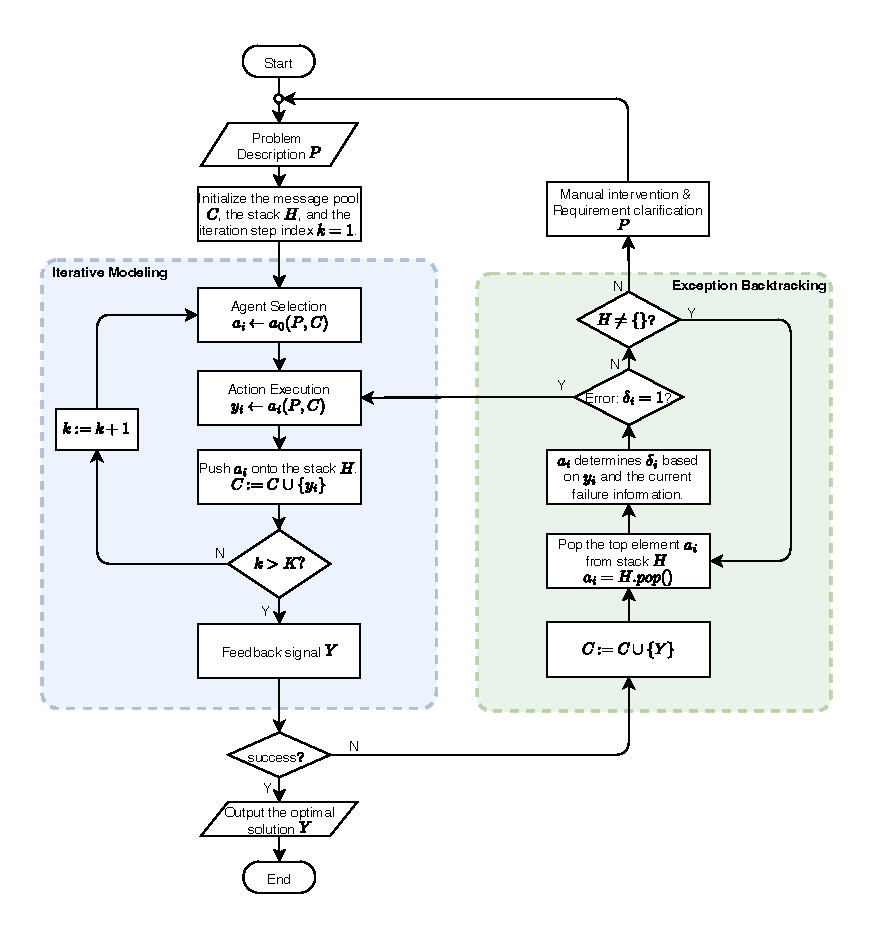
\includegraphics[scale=0.8]{figure/sop_mas_flowchat_black.pdf}
%% Use \caption command for figure caption and label.
\caption{SOP-MAS Flowchart}\label{fig1}
%% https://en.wikibooks.org/wiki/LaTeX/Importing_Graphics#Importing_external_graphics
\end{figure}

It is important to clarify that the proposed SOP-MAS framework is fundamentally designed as an expert-in-the-loop decision support system, rather than a fully autonomous optimization engine. In real-world container logistics operations, particularly in complex, high-stakes scenarios like ECR, the ultimate responsibility for model validity, constraint fidelity, and operational feasibility must rest with domain experts (e.g., logistics planners, operations researchers, or port analysts).

\subsection{Mechanisms for Hallucination Mitigation}

Within the framework of the SOP-MAS methodology, a systematic strategy is adopted to mitigate the pervasive issue of hallucinations in LLMs. This strategy encompasses the integration of prompt engineering, SOP, and a mechanism for exception backtracking and correction.

\begin{enumerate}[label=\arabic*)]
    \item \textbf{Meticulously Designed Prompt Engineering.} To ensure each agent accurately comprehends its role and tasks, and produces outputs that are standardized, this study designs refined prompt templates for each agent. These templates adhere to a unified structure, encompassing key elements such as role definition, principal tasks, input/output specifications, and constraints. By restricting the generation scope and steering the reasoning process through prompt engineering, the LLMs are constrained to produce output strictly in JSON format or in accordance with specific code templates, thereby enforcing structured thinking and minimizing the production of redundant or irrelevant information. Owing to space limitations, this paper will not display all prompts in full but will place their core design logic along with a typical example (e.g., for the ME-Agent) in~\ref{app1}.
    \item \textbf{Constraining Roles by the SOP.} The SOP mitigates risks by clearly defining the responsibilities of each agent and by establishing quality standards for intermediate outputs. Utilizing JSON as the communication protocol between agents inherently restrict each agent's latitude for unstructured "free-form" output, requiring their responses to adhere to specific formats and standards, thereby diminishing the likelihood of generating nonsensical or irrelevant outputs, termed hallucinations. Furthermore, the logical consistency and mathematical correctness of the generated models and code across different agents function as a mechanism for cross-verification.
  \item \textbf{Exception Backtracking and Correction Mechanism.} \deleted{Upon the occurrence of an exception during code execution within the sandbox environment, the TE-Agent retains the error information in the shared message pool.}\changed{Upon the occurrence of an execution or verification failure, the diagnostic evidence is recorded in the shared message pool. If the TE-Agent was selected during the iterative modeling process, its structured execution report—capturing the solver log, error trace, and root-cause analysis—serves as the primary diagnostic artifact; otherwise, the framework records only the bare failure signal from its own code execution.} Concurrently, a stack pop operation is performed on $H$, sequentially popping the topmost agents to check whether the error was caused by the current agent's output. This backtracking mechanism allows for pinpointing the source of errors and facilitates corrective actions, significantly enhancing the robustness of the SOP-MAS framework. By enabling agents to examine and potentially amend their outputs in response to subsequent execution feedback, the system is enabled to autonomously rectify and recover from errors attributable to LLM inaccuracies.
\end{enumerate}

\subsection{Illustrative Example}

\changed{To demonstrate the end-to-end capability of the proposed SOP-MAS framework, we apply it to a single-period, three-port ECR instance. Ports A and B hold surplus containers (100 and 50 TEU, respectively) while port C demands 150 TEU; the unit transportation costs $c_{ij}$ range from 2 to 10 \textyen/TEU. The SOP-MAS is configured with $K{=}5$ collaborating agents, backtracking enabled, DeepSeek-V3-0324 as the backbone LLM, and OR-Tools as the solver. The complete workflow is illustrated in Figure~\ref{fig2}.}

%% Use figure environment to create figures
%% Refer following link for more details.
%% https://en.wikibooks.org/wiki/LaTeX/Floats,_Figures_and_Captions
\begin{figure}[t]%% placement specifier
%% Use \includegraphics command to insert graphic files. Place graphics files in
%% working directory.
\centering%% For centre alignment of image.
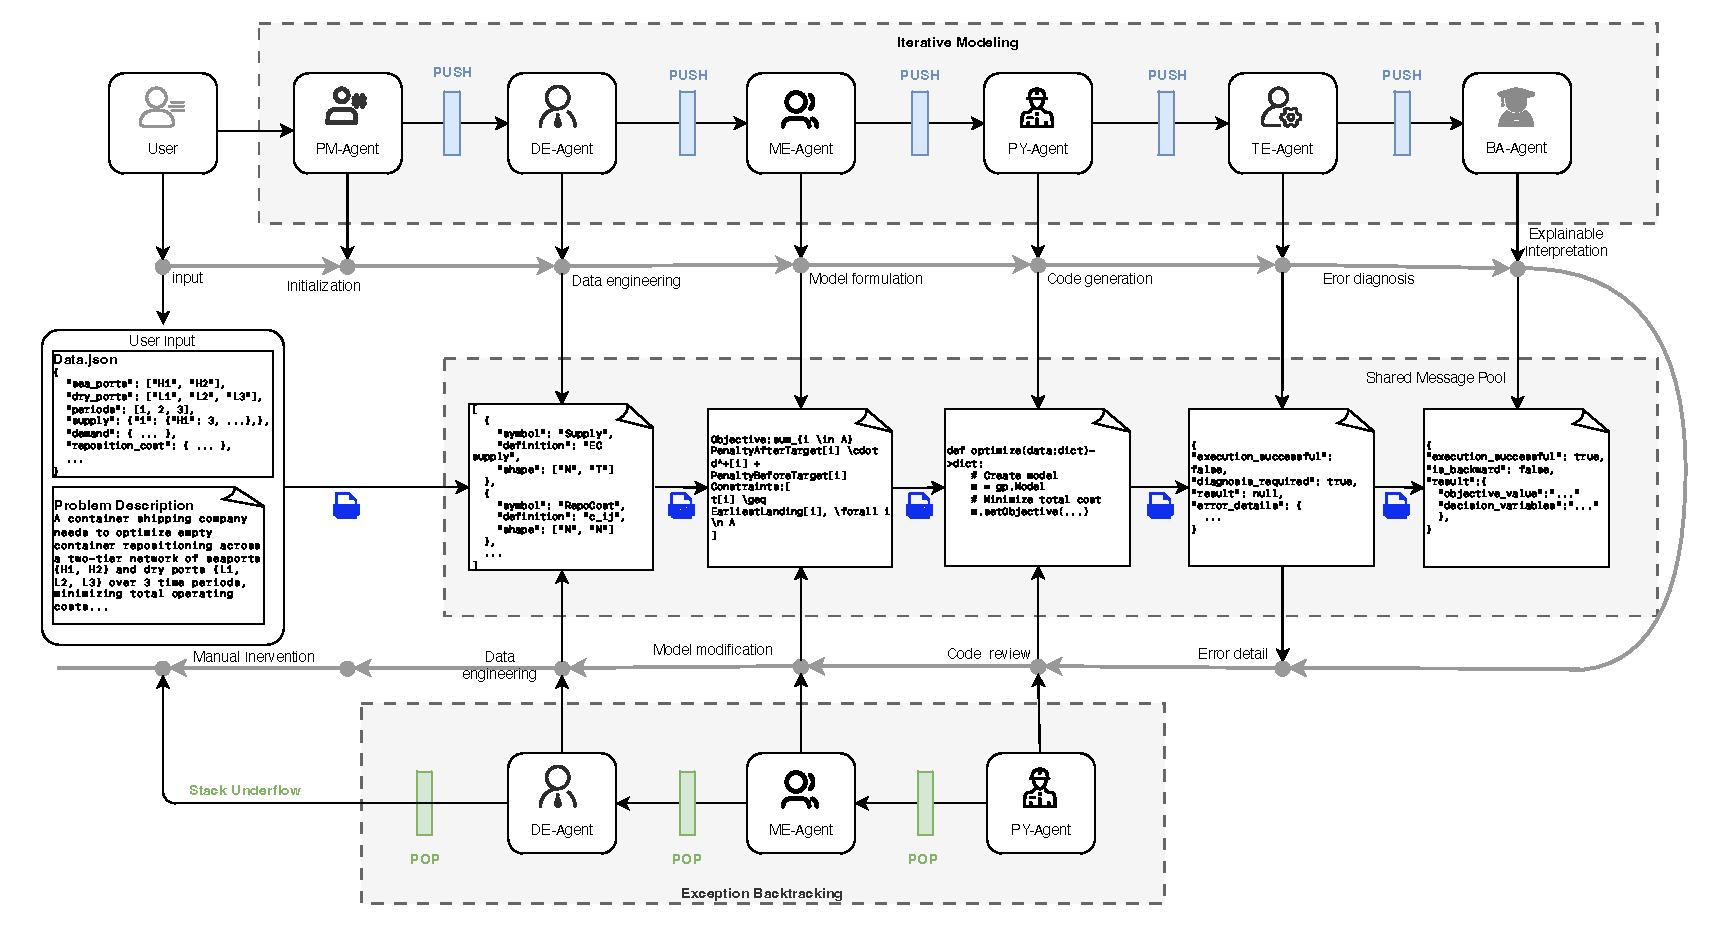
\includegraphics[scale=0.5]{figure/sop_mas_example.pdf}
%% Use \caption command for figure caption and label.
\caption{\changed{End-to-end SOP-MAS workflow on an ECR instance (3 ports, $T{=}1$): from natural-language description to optimal repositioning plan}}\label{fig2}
%% https://en.wikibooks.org/wiki/LaTeX/Importing_Graphics#Importing_external_graphics
\end{figure}

\changed{The PM-Agent orchestrates the five agents in sequence. First, the DE-Agent parses the natural-language problem description and extracts structured parameters: the supply vector $S{=}[100,50,0]$, the demand vector $D{=}[0,0,150]$, and the cost matrix $c_{ij}$. Second, the ME-Agent formulates the LP: $\min \sum_{i,j}c_{ij}x_{ij}$ subject to flow-balance constraints $\sum_j x_{ij}-\sum_j x_{ji}=S_i-D_i$ for each port $i$ and non-negativity $x_{ij}\geq 0$. Third, the PY-Agent generates executable solver code implementing this model. Fourth, the TE-Agent executes the generated code with the actual input data, captures the solver log, and produces a structured diagnostic report; OR-Tools solves the resulting LP in 2 iterations, yielding an optimal total repositioning cost of \textyen650. Fifth, the BA-Agent translates the optimal solution ($x_{AB}{=}100$, $x_{BC}{=}150$, with all other flows equal to zero) into a business-analysis report, correctly stating the optimal total transportation cost of CNY~650, explaining why the low-cost A--B and B--C arcs are selected to satisfy port~C's demand through Port~B as the transfer hub, and clarifying why the expensive direct A--C route and reverse movements remain zero. This small instance therefore provides a transparent sanity check for the interpretation accuracy of the BA-Agent.}

This process—(1) natural-language description, (2) structured modeling, (3) solution-code generation and execution, (4) interpretable results—largely parallels the conventional workflow of mixed-integer programming (MIP) modeling and solution. It highlights the manner in which the MAS assigns individual agents to authentic enterprise roles. Concurrently, the SOP framework bestows unique benefits in the realms of task decomposition, agent scheduling, exception backtracking, and iterative multi-round interaction.

\changed{Should an execution error or incorrect solution occur, the SOP-MAS framework triggers the exception backtracking mechanism. For instance, if the PY-Agent generated code that omitted a flow-balance constraint, the framework's verification stage would detect the resulting incorrect solution, and the TE-Agent would capture the failure signal along with diagnostic evidence in the shared message pool. A stack-based reverse traversal is then performed: agents are popped in last-in-first-out order and each is queried to determine whether the error originated from its output. Upon locating the responsible agent, that agent provides a refined result, which is pushed back onto the stack, and the forward modeling resumes from the corrected step onward using the remaining collaboration rounds. This iterative correction loop continues until a valid solution is obtained or all collaboration rounds are exhausted.}

\section{System Implementation and Experimental Analysis}

The effectiveness of the SOP-MAS method is validated against baseline approaches using publicly available datasets. To identify the optimal hyperparameter configuration, sensitivity analyses are conducted across problem instances of varying scales. All experiments are implemented in Python 3.11.9 on a local machine running Windows 10 Professional, equipped with an Intel i5-4210U CPU and 32 GB of DDR3 memory\changed{. On this machine, the system is exclusively responsible for orchestrating the multi-agent workflow, executing the generated solver code within a sandbox, and managing the shared message pool, while the DeepSeek-V3-0324 model is accessed via a cloud API. For all API calls, \texttt{top\_p} is set to 1.0 (i.e., no nucleus truncation) and \texttt{max\_tokens} is left unspecified to default to the model's maximum output length. This configuration preserves the full output distribution and prevents the artificial truncation of lengthy structured outputs, such as mathematical formulations and solver code.}

\subsection{Comparison with Baseline Methods and Effectiveness Analysis}

To validate the effectiveness of SOP-MAS, a total of 269 instances were selected from the ComplexOR and NLP4LP benchmark datasets. The ComplexOR dataset \citet{xiaoChainofExpertsWhenLLMs2023} is explicitly crafted to provide benchmark tests for complex OR problems, comprising 37 multi-source, heterogeneous scenarios spanning supply chain optimization, scheduling, and warehousing logistics. Each scenario is expert-annotated, including both model formulations and test cases to verify the correctness of generated code. The NLP4LP dataset comprises LP and MIP scenarios, with problem descriptions distinguished by lengthy textual narratives, implicit constraints, and complex data structures (e.g., multi-resource allocation and production scheduling), necessitating domain expertise for accurate mathematical modeling. To strengthen evaluation fidelity, we further refined the annotation of all instances by structuring them into four standardized components:
\begin{enumerate}[label=\arabic*)]
    \item a natural-language problem description (capturing business intent, constraints, and objectives),
    \item structured modeling metadata (including variable definitions, parameter schemas, and constraint templates),
    \item sample input data (e.g., CSV/JSON instances for model instantiation), and
    \item reference optimization outcomes (optimal/near-optimal solutions and solver logs for correctness verification).
\end{enumerate}
This design establishes a closed-loop evaluation framework: SOP-MAS ingests 1) to 3) and is assessed on its ability to reproduce 4) without manual intervention. This structure not only enables rigorous quantitative evaluation but also supports qualitative analysis of modeling fidelity and interpretability, key criteria for real-world deployment.

The performance of SOP-MAS on these instances is evaluated by comparing it against baseline methods on benchmark cases, specifically including the Standard Prompting Method (SPM), CoT, CoE \citep{xiaoChainofExpertsWhenLLMs2023}, and OptiMUS \citep{ahmaditeshniziOptiMUSScalableOptimization2024b}. We adopt DeepSeek-V3-0324 as the backbone LLM \changed{for all methods}, given its leading position among open-weight models. Crucially, this work does not aim to benchmark LLM capabilities; rather, it seeks to evaluate a novel workflow orchestration paradigm—SOP-MAS. Therefore, we do not employ other LLMs, as is consistent with foundational multi-agent frameworks such as AutoGen \citep{wuAutoGenEnablingNextGen2024} and MetaGPT \citep{hongMetaGPTMetaProgramming2023a}. \changed{All baselines were evaluated under the same DeepSeek-V3-0324 backbone and identical hardware conditions to ensure a fair comparison.}

Similarly, OR-Tools is employed as the solver, an open-source optimization engine widely used for MIP/LP prototyping in academia and industry. The PY-Agent generates solver-agnostic Python code; adapting the same prompt template to OR-Tools or CPLEX requires only minimal syntactic substitution (e.g., changing the solver creation call), confirming the framework's portability. Thus, validation under different solvers would assess solver characteristics rather than the efficacy of SOP-MAS itself, which lies beyond the scope of this study.

Following the metrics proposed in \citet{xiaoChainofExpertsWhenLLMs2023}, the evaluation was performed utilizing Compile-Time Errors (CER), Run-Time Errors (RER), and Accuracy Rate (AR). \changed{For each test instance $i \in \{1,\dots,N\}$, let $c_i \in \{0,1\}$ indicate successful compilation, $r_i \in \{0,1\}$ indicate execution without runtime errors, $s_i$ denote the solver status, $z_i$ denote the objective value returned by the generated code, and $\hat z_i$ denote the ground-truth optimal objective value. CER and RER are defined as}
\begin{equation}
\changed{\mathrm{CER}=\frac{1}{N}\sum_{i=1}^{N}\mathbf{1}(c_i=0).}
\end{equation}


\begin{equation}
\changed{ \mathrm{RER}=\frac{\sum_{i=1}^{N}\mathbf{1}(c_i=1,\; r_i=0)}{\sum_{i=1}^{N}\mathbf{1}(c_i=1)}. }
\end{equation}

\changed{To distinguish executable correctness from mathematical correctness, we further define}
\begin{equation}
\changed{a_i=\mathbf{1}\!\left(c_i=1,\; r_i=1,\; s_i=\mathrm{Optimal},\; \frac{|z_i-\hat z_i|}{\max(1,|\hat z_i|)}\le \varepsilon\right).}
\end{equation}
\changed{The accuracy rate is then defined as}
\begin{equation}
\changed{\mathrm{AR}=\frac{1}{N}\sum_{i=1}^{N} a_i.}
\end{equation}
\changed{In this study, $\varepsilon = 10^{-6}$.} Each algorithm was executed five times with $K=5$. Mean results are summarized in Table~\ref{tab:benchmark}.

%% Refer following link for more details.
%% https://en.wikibooks.org/wiki/LaTeX/Mathematics
%% https://en.wikibooks.org/wiki/LaTeX/Advanced_Mathematics

%% Use a table environment to create tables.
%% Refer following link for more details.
%% https://en.wikibooks.org/wiki/LaTeX/Tables
\begin{table}[t]%% placement specifier
%% Use tabular environment to tag the tabular data.
%% https://en.wikibooks.org/wiki/LaTeX/Tables#The_tabular_environment
\caption{Comparison of SOP-MAS and Baseline Algorithms}\label{tab:benchmark}

\centering%% For centre alignment of tabular.
\begin{tabular}{l c c c}
\hline
Baseline & CER & RER & AR \\
\hline
Standard Prompting Method (SPM) & 7.67\% & 11.81\% & 48.08\% \\
Chain-of-Thought (CoT) & 7.32\% & 10.83\% & 52.26\% \\
Chain-of-Experts (CoE) & 4.18\% & 5.77\% & 62.37\% \\
OptiMUS & 3.14\% & 4.51\% & 77.35\% \\
SOP-MAS & 1.39\% & 2.91\% & 86.59\% \\
\hline
\end{tabular}
\end{table}


The findings suggest that the SPM methodology exhibits the lowest accuracy among all evaluated approaches, mainly due to its black-box reasoning which concentrates solely on the final solution, while neglecting the model's intermediate reasoning steps. This deficiency may result in imprecise outputs when tackling complex problems. In contrast, the CoT method, by employing stepwise reasoning, enhances the model's interpretability and displays better performance on complex instances, realizing \deleted{an increase in accuracy by 8.69\%}\changed{an increase in accuracy from 48.08\% to 52.26\% (a relative improvement of 8.69\%)} over SPM. Both the CoE and OptiMUS methods reasonably capitalize on multi-agent collaboration to address complex optimization problems effectively. Notably, the proposed SOP-MAS method achieves the highest accuracy among all baseline approaches.

Notably, the SOP-MAS framework achieves an accuracy rate of 86.59 percent, which falls short of perfect automation. This outcome is neither unexpected nor undesirable; rather, it reflects the intrinsic complexity of real-world operational modeling. In practice, even seasoned SCM experts seldom produce a fully correct MIP model on the first attempt. Instead, model development routinely proceeds through multiple cycles of refinement, guided by feasibility diagnostics, sensitivity testing, and iterative feedback from domain stakeholders. Consistent with this reality, SOP-MAS is deliberately designed as a human-in-the-loop decision support tool rather than a fully autonomous optimizer. Its primary objective is to \deleted{shorten the expert-centered formulation cycle}\changed{accelerate the expert modeling workflow, which in practice often spans hours or even weeks for complex real-world problems,} by automating routine tasks such as data parsing, constraint drafting, and code generation, while simultaneously surfacing potential inconsistencies or violations for expert review. \changed{Final validation, business-rule checking, and strategic acceptance remain the responsibility of human experts.} In doing so, the framework shifts human effort away from mechanical implementation toward high-value activities such as model validation, business logic verification, and strategic refinement.

\subsection{Sensitivity Analysis of LLM Parameters}

\changed{Within the SOP-MAS framework, the maximum collaboration count $K$ of the PM-Agent governs the depth and breadth of the workflow by modulating the number of agent invocations. Among the six agents, the temperatures of the ME-Agent and PY-Agent, denoted as $t_{ME}$ and $t_{PY}$, are the primary determinants of solution accuracy, because these two agents are directly responsible for mathematical model construction and executable code generation, respectively. The temperatures of the remaining agents (DE-Agent, PM-Agent, TE-Agent, and BA-Agent) have a relatively minor impact on the optimization outcome, as validated by the ablation study in Section~4.3. Temperature significantly affects the optimization modeling and solution outputs generated by the agents: elevated temperatures foster more innovative solutions, while reduced temperatures bolster deterministic reasoning, ensuring stability and compliance of the outputs. This trade-off between precision and creativity mandates meticulous calibration of the temperature parameters tailored to specific task scenarios.}

In order to systematically evaluate the effects of parameter configurations on the performance of multi-agent collaboration, a three-dimensional sensitivity analysis framework was developed using the benchmark instance set. The exception backtracking mechanism was deactivated (\deleted{is\_backward=False}\changed{\texttt{is\_backward} = \texttt{False}}) to eliminate any confounding variables. A grid search was performed over the parameters $K \in [2, 5]$ and $t_{ME}, t_{PY} \in \{0.2, 0.4, 0.8, 1.0\}$, utilizing AR as the evaluation metric to identify the optimal parameter combination. The results are shown in Figure~\ref{fig3}.

%% Use figure environment to create figures
%% Refer following link for more details.
%% https://en.wikibooks.org/wiki/LaTeX/Floats,_Figures_and_Captions
\begin{figure}[t]%% placement specifier
%% Use \includegraphics command to insert graphic files. Place graphics files in
%% working directory.
\centering%% For centre alignment of image.
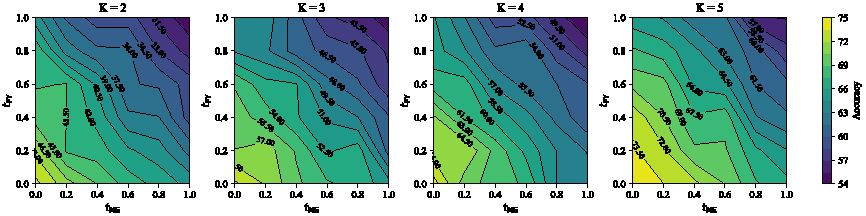
\includegraphics[scale=0.9]{figure/figure_sensitivity_analysis.pdf}
%% Use \caption command for figure caption and label.
\caption{Faceted Contour Plot of Parameter Sensitivity Analysis}\label{fig3}
%% https://en.wikibooks.org/wiki/LaTeX/Importing_Graphics#Importing_external_graphics
\end{figure}

The PM-Agent orchestrates its constituent agents in accordance with the predefined maximum collaboration threshold $K$ throughout the iterative modeling process. This organization consequently influences the comprehensive scope and extent of the workflow. In instances where $K$ is minimal, the system depends on a limited number of agents to facilitate rapid decision-making, which is appropriate for tasks requiring immediate attention. Conversely, an augmentation in $K$ allows for the incorporation of additional domain-knowledge verification steps, rendering it more suitable for highly complex business scenarios. Notably, as $K$ attains the value of 5, there is a notable enhancement in accuracy, indicating that multi-agent collaboration fosters specialization, with each agent concentrating on a distinct domain.

In contrast, an increase in the parameters $t_{ME}$ and $t_{PY}$ results in declines in accuracy. For both the ME-Agent and PY-Agent, elevated temperatures within the context of mathematical modeling and programming are associated with reduced accuracy. This occurs because lower temperatures substantially limit the randomness in generated outputs, thus ensuring logical rigor and syntactical precision. This is critical for tasks requiring precise derivation, such as mathematical formulae, or strict syntax, such as programming tasks, where sustaining accuracy may slightly constrain creativity but effectively diminishes error rates and enhances development efficiency.

\subsection{Ablation Study}
An ablation study was conducted to assess the contribution of each agent within SOP-MAS and the effectiveness of the collaborative mechanisms. The fundamental operations of SOP-MAS in addressing optimization challenges are rooted in mathematical modeling and code execution. Consequently, this study examines system performance through the selective removal of certain agents or restricting the exception-backtracking mechanism. The experimental groups are defined as follows:

\begin{enumerate}[label=\arabic*)]
    \item \textbf{Group~1 $(a_{ME}, a_{PY})$:} Solely comprises the ME-Agent and PY-Agent, with exception backtracking deactivated, to assess the significance of collaboration among multiple agents.

    \item \textbf{Group~2 $(a_{PM}, a_{DE}, a_{ME}, a_{PY}, a_{TE})$:} Excluding the BA-Agent whilst permitting exception backtracking to examine the role of the BA-Agent.

    \item \textbf{Group~3 $(a_{PM}, a_{ME}, a_{PY}, a_{TE}, a_{BA})$:} The DE-Agent is excluded, with exception backtracking enabled, to evaluate the significance of structured modeling information.

    \item \textbf{Group~4 $(a_{PM}, a_{DE}, a_{ME}, a_{PY}, a_{BA})$:} The TE-Agent is omitted to examine the interaction between testing and exception backtracking, while exception backtracking remains enabled. In this group, the absence of the TE-Agent results in the non-generation of diagnostic reports. \deleted{However, the exception backtracking mechanism remains active, enabling each agent to perform self-checks on its output to detect probable errors.}\changed{However, the exception backtracking mechanism remains active because it is triggered by SOP-MAS execution or verification failure rather than by TE-Agent selection itself. In this setting, previously selected agents are queried in reverse order on the basis of the failure signal returned by the execution and verification stage, without the structured diagnostic report normally provided by the TE-Agent.}

    \item \textbf{Group~5 $(a_{PM}, a_{DE}, a_{ME}, a_{PY}, a_{TE}, a_{BA})$:} All six agents are retained, while exception backtracking is disabled, in order to examine the effect of the exception-backtracking mechanism on system performance.
\end{enumerate}
The entirety of SOP-MAS functions as the control group for assessing performance benchmarks. Within this context, the symbol "+" indicates that exception backtracking is activated, whereas "-" denotes its deactivation. The experimental results are presented in Table~\ref{tab:ablation}.

\begin{table}[htbp]
    \centering
    \caption{Ablation Study}\label{tab:ablation}
    \begin{tabular}{lccc}
        \hline
        Group No. & CER & RER & AR \\
        \hline
        \changed{Group1 ($-$)} & 6.27\% & 9.80\% & 57.84\% \\
        \changed{Group2 ($+$)} & 1.74\% & 2.55\% & 82.58\% \\
        \changed{Group3 ($+$)} & 1.74\% & 3.68\% & 73.17\% \\
        \changed{Group4 ($+$)} & 1.44\% & 2.09\% & 84.32\% \\
        \changed{Group5 ($-$)} & 3.48\% & 4.53\% & 69.69\% \\
        \changed{Control Group ($+$)} & 1.39\% & 2.91\% & 86.59\% \\
        \hline
    \end{tabular}
\end{table}


In Group 1, which consists exclusively of $a_{ME}$ and $a_{PY}$, there is \deleted{a 28.75\% reduction in accuracy}\changed{a decrease in accuracy from 86.59\% to 57.84\%} compared to the control group. This decline highlights the significance of multi-agent collaboration in SOP-MAS for tackling complex optimization problems. In Group 2, the removal of the BA-Agent results in an accuracy level of 82.58\%, indicating that the BA-Agent exerts a minimal influence on overall accuracy. This is attributed to the position of the BA-Agent at the terminal part of the workflow, where its primary function is the interpretation and packaging of previously obtained results. Consequently, its absence does not compromise the accuracy of front-end modeling and problem-solving but affects solely the presentation and clarity of the final output delivered to the user. The experimental metric, Accuracy Rate (AR), inherently fails to account for the BA-Agent's contribution, and this limitation should be clearly indicated. \changed{Because the BA-Agent operates after solution generation, removing it has limited effect on AR even though it reduces the interpretability of the final output. Its main contribution is to translate solver outputs into interpretable business reports for end users, as illustrated by the three-port example in Section~3.4 and the empirical case in Section~\ref{sec:results_analysis}, where it explains routing decisions, decomposes total cost, and provides managerial recommendations. A formal qualitative evaluation of this interpretive contribution is left for future work.} In Group 3, the removal of the DE-Agent results in \deleted{a 13.42\% reduction in accuracy}\changed{a decrease in accuracy from 86.59\% to 73.17\%} relative to the control group, demonstrating that structured modeling information is instrumental for the ME-Agent in precisely delineating problem parameters. \deleted{Group 4 indicates that the exclusion of the TE-Agent still results in a relatively high accuracy, as the testing agent is capable of providing detailed error information, and errors can be rectified via the exception-backtracking mechanism.}\changed{Group 4 still achieves a relatively high accuracy, but it remains below the control group. This result suggests that exception backtracking preserves substantial recovery capability even when the TE-Agent is excluded, while the TE-Agent provides more detailed runtime evidence for diagnosing the source of failure.} This observation is consistent with the findings in Group 5, where disabling exception backtracking results in a significant decline in accuracy.

\subsection{Computational Efficiency Analysis}

To provide a comprehensive performance analysis, we present a detailed evaluation of the proposed LLM-MAS framework. This analysis encompasses 25 representative cases that span a range of problem scales, randomly sampled from the total pool of 269 instances. The findings are summarized in Figure~\ref{fig4}, illustrating the roles of each agent, their average task completion times, and the variability thereof, all measured in seconds.

%% Use figure environment to create figures
%% Refer following link for more details.
%% https://en.wikibooks.org/wiki/LaTeX/Floats,_Figures_and_Captions
\begin{figure}[t]%% placement specifier
%% Use \includegraphics command to insert graphic files. Place graphics files in
%% working directory.
\centering%% For centre alignment of image.
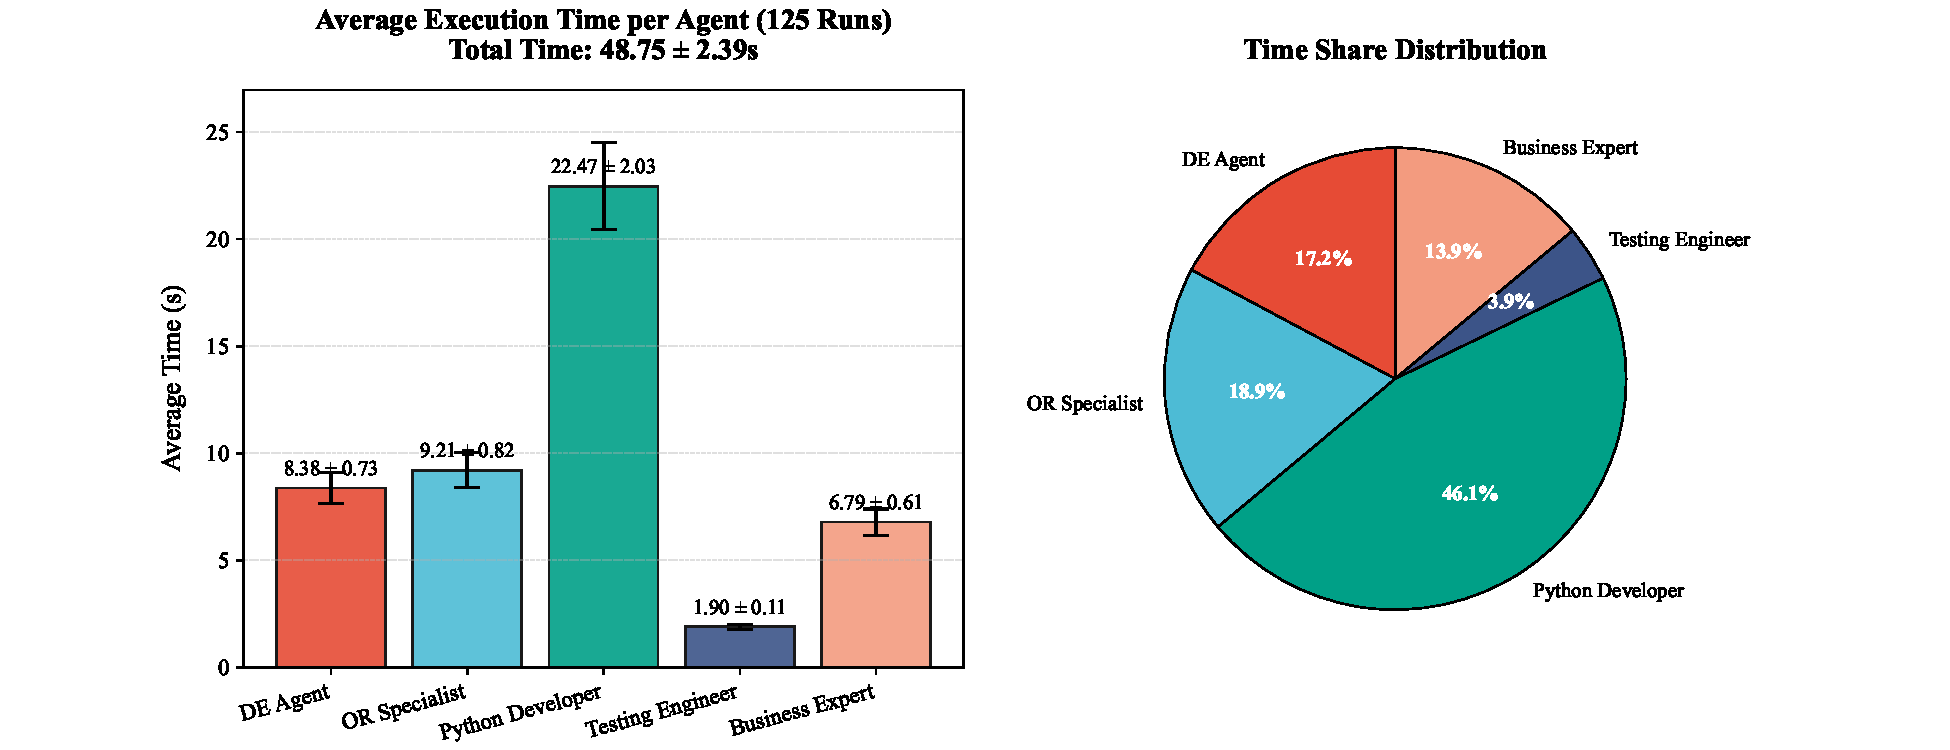
\includegraphics[scale=0.4]{figure/agent_runtime_combined.pdf}
%% Use \caption command for figure caption and label.
\caption{Average Execution Time and Time Share Distribution}\label{fig4}
%% https://en.wikibooks.org/wiki/LaTeX/Importing_Graphics#Importing_external_graphics
\end{figure}

Our experimental results indicate that the PY-Agent experiences the longest average processing time among all agents, taking approximately 22.47 seconds per task with a standard deviation of 2.03 seconds. This extended duration likely reflects the complexity and variability inherent in coding processes. Conversely, the TE-Agent completes tasks in the shortest average time, requiring only about 1.90 seconds per task, with a notably small standard deviation of 0.11 seconds. This indicates a high level of consistency and efficiency in executing testing tasks.

The other agents, including the DE-Agent (8.38 ± 0.73 seconds), ME-Agent (9.21 ± 0.82 seconds), and BA-Agent (6.79 ± 0.61 seconds), also demonstrate efficient performance with acceptable variances, contributing to the overall robustness and practical deployability of the SOP-MAS framework.

Aggregating across all stages, the average end-to-end runtime per instance is approximately 48.75 seconds (sum of mean agent times), with an estimated total standard deviation of ~2.4 seconds (propagated from individual variances). This sub-minute latency demonstrates that the framework is well-suited for tactical decision-making scenarios in port operations, where planning horizons typically span hours or days rather than real-time milliseconds. \changed{The modeling runtime of SOP-MAS is dominated by LLM API calls rather than problem scale. This scale‑independence stems from the architectural separation between the abstract symbolic problem description (parameters, variables, constraints) and the concrete numerical data. Because the problem description is expressed in index notation (e.g., $i \in I$, $t \in T$), the model structure generated by the ME‑Agent and the code template produced by the PY‑Agent remain invariant to the number of ports or time periods. Consequently, the sub‑minute modeling overhead of SOP‑MAS stays constant as problem size increases. The actual problem scale, manifested in the number of decision variables and constraints, only affects the solver execution phase, whose scalability has been extensively validated by the OR community. This separation of concerns makes SOP‑MAS suitable for industrial‑scale applications where the computational bottleneck resides in the solver, not in the modeling process.} \changed{Furthermore, the per-agent times reported above are end-to-end latencies that inherently bundle LLM inference, API communication, and inter-agent coordination into one measurement. Since agents execute sequentially with lightweight message-pool operations at each handoff, the multi-agent coordination overhead is negligible relative to the LLM inference time; the dominant factor is the reasoning complexity of individual agents. The reported 48.75\,s should be interpreted as the time required to generate an executable initial model, rather than the full human modeling cycle, which additionally involves requirement clarification, iterative formulation revision, debugging, and stakeholder validation.}

\section{Empirical Analysis}

This section selects ECR as the empirical testbed not only because it epitomizes the structural inefficiencies pervasive in global container logistics, but more importantly because it represents a high-stakes, data-rich, and operationally nuanced problem that demands both mathematical rigor and business interpretability, precisely the dual requirements our SOP-MAS framework is designed to fulfill. Unlike generic optimization benchmarks, real-world ECR involves intricate trade-offs among transportation cost, multimodal transport, and contractual obligations across multiple stakeholders, making it an ideal domain for evaluating whether AI-driven modeling can transition from theoretical promise to industrial utility. Within this context, the Northeastern Hinterland of the Liaoning Coastal Port Cluster, encompassing major ports such as Dalian, Yingkou, and Dandong, and their inland logistics networks across Liaoning, Jilin, and Heilongjiang provinces, is chosen as the geographic focus for three compelling reasons.

\subsection{Case Setup and Data Sources}

The empirical analysis examines the coastal port cluster of Liaoning and its hinterland in Northeast China. Dalian Port serves as a hub for the northeastern economic region, which encompasses the three provinces of Liaoning, Jilin, and Heilongjiang, as well as the four eastern leagues of Inner Mongolia. Yingkou Port and Dalian Port compose a dual-core driving structure. Dandong Port functions as the logistics gateway for the eastern part of Northeast China. Those three ports share overlapping hinterlands in the inland Northeast, forming key nodes for sea–rail intermodal transportation. Through differentiated strategic positioning, Dalian Port emphasizes international transshipment, Yingkou Port concentrates on low-cost land transport, and Dandong Port specializes in the eastern border region; together, the three ports fulfill complementary roles. The port hinterlands are illustrated in Figure~\ref{fig:port_hinterland_map}.


The examination of empty container repositioning within this regional port cluster entails the involvement of high-dimensional discrete decision variables, constraints specific to the domain, and complex model transformations. This setting serves as an exemplary testbed to evaluate the robustness and generalization capability of the proposed SOP-MAS method in complex, real-world scenarios.

%% Use figure environment to create figures
%% Refer following link for more details.
%% https://en.wikibooks.org/wiki/LaTeX/Floats,_Figures_and_Captions
\begin{figure}[t]%% placement specifier
%% Use \includegraphics command to insert graphic files. Place graphics files in
%% working directory.
\centering%% For centre alignment of image.
\includegraphics[scale=0.6]{figure/port_hinterland_map.pdf}
%% Use \caption command for figure caption and label.
\caption{Port Hinterland Map}\label{fig:port_hinterland_map}
%% https://en.wikibooks.org/wiki/LaTeX/Importing_Graphics#Importing_external_graphics
\end{figure}

The distances between each port within the Liaoning coastal port cluster and the corresponding dry ports in the Northeastern hinterland are summarized in Table~\ref{tab:seaport_repositioning}. This investigation adopts a planning horizon of five periods, each with a duration of seven days. Distances between each seaport and dry port are listed in Table~\ref{tab:port_hinterland_distance}, while inter-dry-port distances are given in Table~\ref{tab:inter_dryport_distance}. As articulated by \citet{caiJointOptimizationEmpty2024}, the freight rates applicable to empty container transportation by maritime, road, and rail modalities are determined to be 0.8, 4.5, and 1.8 CNY per TEU per kilometer, respectively. The leasing expense for empty containers at seaports is determined to be 4,000 CNY per TEU, with the storage cost for these containers at seaports set at 10 CNY per TEU daily, whereas the average holding cost at dry ports is established at 5 CNY per TEU daily. The supply and demand dynamics of empty containers at each node per period follow a normal distribution, as detailed by \citet{caiJointOptimizationEmpty2024}, with specific details provided in Table~\ref{tab:ec_demand_supply}. Tables~\ref{tab:seaport_repositioning}, \ref{tab:port_hinterland_distance}, \ref{tab:inter_dryport_distance}, and~\ref{tab:ec_demand_supply} can be found in Appendix~\ref{app2}.


\subsection{Problem Description}

The ECR network is represented by a directed graph $G=\left(\mathcal{N},E\right)$, where the node set $\mathcal{N}$ consists of two distinct categories: the seaport set $\mathcal{P}$ and the dry port set $\mathcal{L}$, such that $\mathcal{N}=\mathcal{P}\cup\mathcal{L}$. \changed{Let $T=\{1,2,\ldots,|T|\}$ denote the set of time periods in the planning horizon, indexed by $t \in T$.} The edge set $E$ symbolizes the routes for the repositioning of empty containers, including pathways between seaports, between dry ports, and between seaports and dry ports. A parameter $\lambda_{ij}$ is introduced to describe the hinterland affiliation between seaport $i\in \mathcal{P}$ and dry port $j\in \mathcal{L}$. Specifically, $\lambda_{ij}=1$ indicates that dry port $j$ belongs to the hinterland of seaport $i$, thereby permitting the repositioning of empty containers between them. In instances where two dry ports $j_1,j_2\in \mathcal{L}$ are associated with the same seaport $i\in \mathcal{P}$ ($\lambda_{ij_1}=\lambda_{ij_2}=1$), direct repositioning of empty containers between these dry ports is permitted, reflecting the capability for intra-regional collaborative transport. The supply of empty containers primarily originates from the conversion of inbound laden containers. Specifically, laden containers arriving at seaport $i\in \mathcal{P}$ in the preceding period are converted into the empty container supply $Q_i^t$ for the current period; similarly, laden containers that arrived at dry port $j\in \mathcal{L}$ in the preceding period are converted into the empty-container supply $Q_j^t$ for the current period. Correspondingly, the outbound laden containers from node $i\in \mathcal{P}\cup\mathcal{L}$ constitute its empty container demand, $D_i^t$. Each seaport and dry port node is subject to a maximum storage capacity $U_i^{\max}$ and incurs a per-period holding cost $c_i^\text{hold}$. When a node experiences an empty container shortage, the demand can be accommodated by repositioning containers from alternative nodes or through the leasing of containers from external providers. The cost associated with repositioning a unit empty container from node $i$ to node $j$ utilizing transport mode $m\in \mathcal{M}$ is denoted as $c_{ijm}^\text{repos}$, with a maximum transport capacity of $F_{ijm}^{\max}$ for each mode. Leasing a container incurs a cost per unit, represented by $c_i^\text{rent}$ at node $i$.
In the context of container shipping companies, the issue of repositioning empty containers is conceptualized within a two-tier network encompassing both seaports and dry ports over multiple time periods. The primary aim is to minimize the aggregate operational expenses, encompassing costs related to repositioning, storage, and leasing. To simplify the model and enhance the ease of its analysis and resolution, the subsequent assumptions have been established:

\begin{enumerate}[label=\arabic*)]
    \item The movement of empty containers may occur among seaports, between seaports and dry ports, as well as among dry ports.
    \item Both seaports and dry ports can store empty containers, with the inventory in any period not exceeding the maximum storage capacity.
    \item Seaports and dry ports have the capability to lease a virtually unrestricted quantity of containers during the present operation period.
    \item As container shipping services generally adhere to a predetermined weekly schedule, this research employs a 7-day (one-week) decision period as the fundamental unit of planning.
\end{enumerate}

\changed{To keep the main text focused on the problem setting and empirical analysis, the complete mathematical formulation used in the ECR case is provided in Appendix~\ref{app3}, while the key decision logic, variables, and operational assumptions are summarized above.}

\subsection{Results Analysis}\label{sec:results_analysis}

Based on the ECR problem setting described in Section~5.2 and the data presented in Section~5.1, the SOP-MAS framework was employed for end-to-end optimization.

\changed{Under the sea–land coordination scenario (Scenario~1), wherein hinterland lateral repositioning is permitted, the optimal total cost over the five-period planning horizon is CNY~1,190,336, comprising repositioning costs of CNY~763,966, holding costs of CNY~30,870, and leasing costs of CNY~395,500, as summarized in Table~\ref{tab:cost_summary}.}

\changed{To evaluate the benefits of hinterland lateral repositioning, a comparative analysis was conducted under the scenario without inter-dry-port exchange (Scenario~2), as illustrated in Figure~\ref{fig:cost_comparison}. As shown in Table~\ref{tab:cost_summary}, the total cost increases from CNY~1,190,336 to CNY~1,355,388 (+13.86\%). This increase is primarily driven by the repositioning costs, which rise from CNY~763,966 to CNY~925,238 (+21.11\%). Within the repositioning category, the sea--land repositioning cost surges from CNY~594,952 to CNY~864,910 (+45.38\%), as the network must compensate for the loss of hinterland lateral flows (CNY~110,718 reduced to zero) by routing more containers through the sea--dry corridors. Furthermore, the exacerbated difficulty in empty container flows leads to a greater number of containers failing to arrive at shortage seaports in a timely manner, which in turn increases the leasing demand at the affected seaports from CNY~395,500 to CNY~406,000 (+2.66\%). Overall, enabling hinterland lateral repositioning yields a 12.18\% reduction in total operational costs.}

\changed{
\begin{table}[htbp]
\centering
\caption{Comparison of cost structures under the two scenarios (CNY)}
\label{tab:cost_summary}
\small
\setlength{\tabcolsep}{6pt}
\renewcommand{\arraystretch}{1.18}
\begin{tabular}{@{}>{\raggedright\arraybackslash}p{0.46\linewidth} r r r@{}}
\toprule
\textbf{Cost component} & \textbf{Scenario~1} & \textbf{Scenario~2} & \textbf{Change} \\
\midrule
\textbf{Repositioning cost} & \textbf{763,966} & \textbf{925,238} & +21.11\% \\
\hspace{1.2em}Seaport feeder repositioning & 58,296 & 60,328 & +3.47\% \\
\hspace{1.2em}Sea--land repositioning & 594,952 & 864,910 & +45.38\% \\
\hspace{1.2em}Hinterland lateral repositioning & 110,718 & 0 & \textemdash{} \\
\addlinespace[2pt]
Holding cost & 30,870 & 24,150 & $-$21.86\% \\
Leasing cost & 395,500 & 406,000 & +2.66\% \\
\midrule
\textbf{Total cost} & \textbf{1,190,336} & \textbf{1,355,388} & +13.86\% \\
\bottomrule
\end{tabular}
\end{table}
}

\changed{Beyond the numerical comparison in Table~\ref{tab:cost_summary}, the BA-Agent converts the large-scale solver output for Scenario~2 into a structured business report. Specifically, it identifies the total cost as CNY~1,355,388 and attributes 68.26\% to repositioning (CNY~925,238), 29.95\% to leasing (CNY~406,000), and 1.78\% to holding (CNY~24,150). It further highlights the dominant supply and receiving hubs, identifies shortage-prone inland nodes, and recommends prioritizing the Yingkou--Dalian repositioning corridor, securing long-term leasing agreements in inland shortage locations, and clearing stagnant inventories in peripheral nodes. This example illustrates how the BA-Agent transforms a mathematically optimal solution into an actionable managerial interpretation.}

%% Use figure environment to create figures
%% Refer following link for more details.
%% https://en.wikibooks.org/wiki/LaTeX/Floats,_Figures_and_Captions
\begin{figure}[t]%% placement specifier
%% Use \includegraphics command to insert graphic files. Place graphics files in
%% working directory.
\centering%% For centre alignment of image.
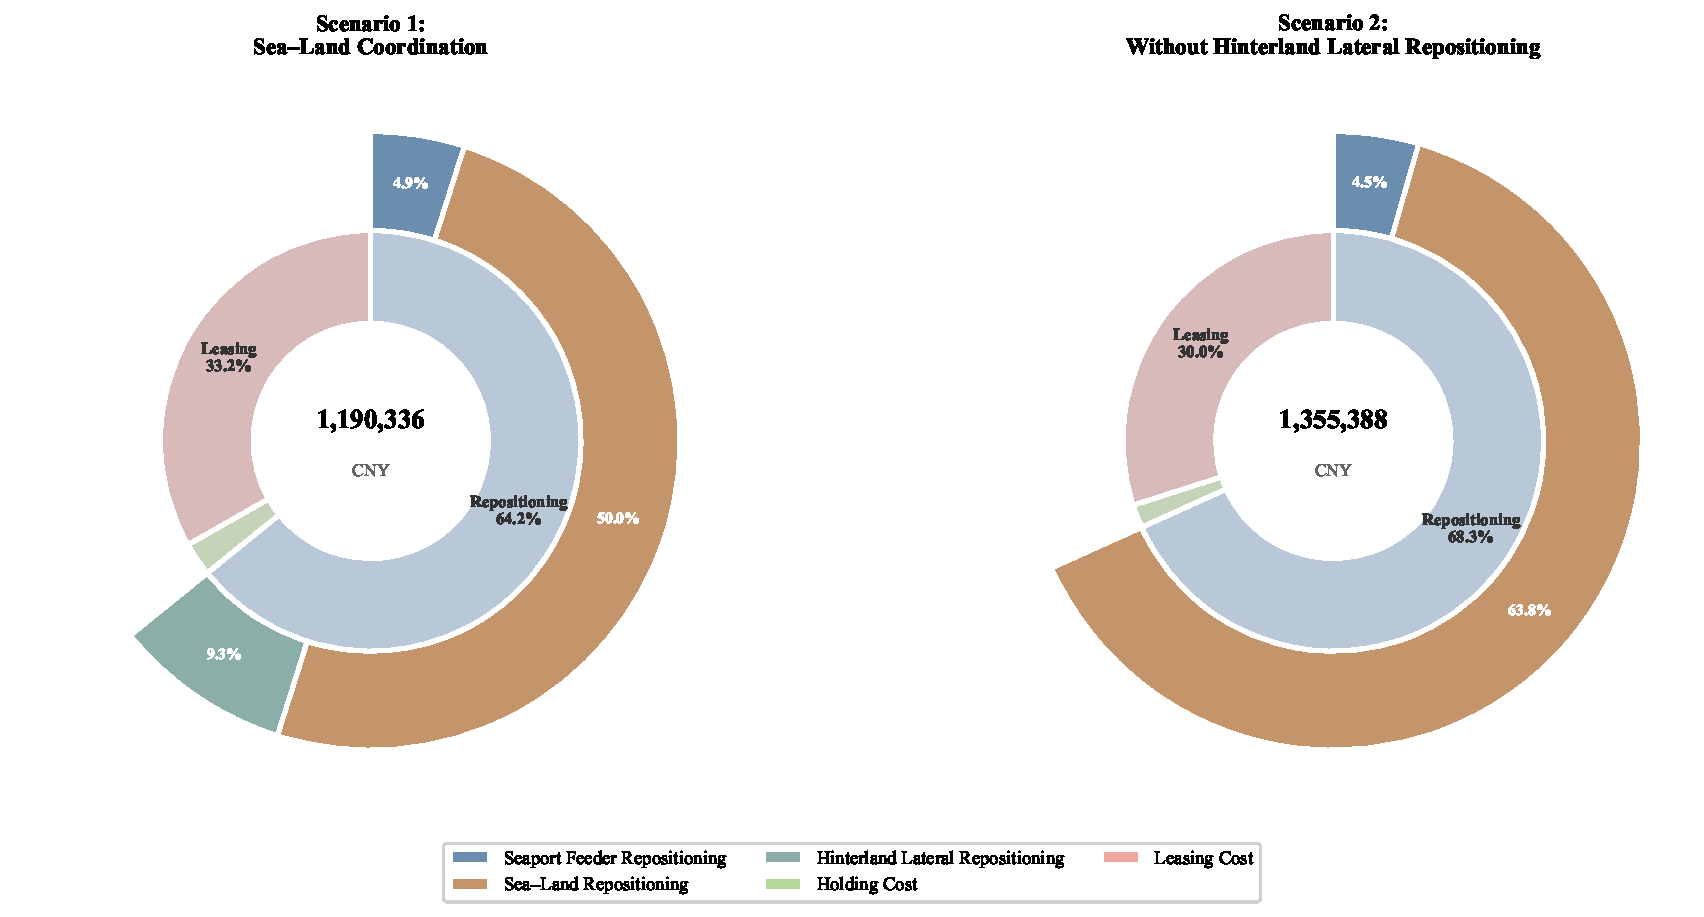
\includegraphics[scale=0.4]{figure/cost_style4_sunburst.pdf}
%% Use \caption command for figure caption and label.
\caption{Cost Comparison}\label{fig:cost_comparison}
%% https://en.wikibooks.org/wiki/LaTeX/Importing_Graphics#Importing_external_graphics
\end{figure}

\section{Conclusions}

In order to address the limitations associated with MIP, which predominantly relies on domain experts and requires problem-specific customization, this study introduces a decision-support framework titled SOP-MAS. This framework integrates large language models with multi-agent theory. The proposed framework facilitates end-to-end optimization by translating natural language descriptions of business optimization problems into actionable business solutions, thereby substantially reducing the application threshold of MIP. To mitigate hallucination issues and the black-box nature of LLM-based decision-making, this study introduces carefully designed prompts, an orchestrated workflow based on standard operating procedures, and an exception-backtracking mechanism to enhance interpretability.

The effectiveness of the approach was validated through comparisons with multiple baseline methods on the ComplexOR and NLP4LP benchmark datasets, achieving an accuracy of 86.59\%. SOP-MAS was subsequently employed to address the empty container repositioning challenge in the Liaoning coastal port cluster–Northeast hinterland context, \deleted{leading to a 12.18\% reduction in repositioning costs for the shipping company.}\changed{leading to a 12.18\% reduction in total operational costs for the shipping company.} This application notably curtailed modeling and solution times, expedited prototype development, and furnished scalable decision support amid evolving business rules.

At present, LLM-based AI agents are incapable of fully supplanting human experts; domain-specific agents primarily serve as auxiliary AI copilots. Consequently, the proposed method has been experimentally validated solely within the context of MIP and cannot entirely substitute human expertise. \deleted{As training parameters and scale increase, pre-trained LLMs are anticipated to achieve further advancements in capability. By integrating general-purpose LLMs with customized knowledge bases, the cost associated with decision-making can be significantly reduced. From the perspective of shipping companies, which occupy a central role in the empty container repositioning process, the proposed approach can be further extended to support additional stakeholders, including seaports, dry ports/inland container yards, shippers/customers, and third-party leasing companies.}\changed{Several promising directions merit further investigation. First, extending the SOP-MAS framework to more complex optimization paradigms, such as stochastic programming, robust optimization, and multi-objective optimization, would broaden its applicability to real-world ECR scenarios involving demand uncertainty, disruption risks, and conflicting stakeholder objectives. Second, deploying the framework in interactive, human-in-the-loop settings would allow logistics practitioners to intervene at agent handoff points (e.g., validating the OR Specialist's mathematical model before it is passed to the Python Developer), enabling iterative refinement and supporting a broader set of stakeholders, including seaports, dry ports, shippers, and third-party leasing companies, within the container supply chain. Third, while the CER, RER, and AR metrics rigorously evaluate the optimization core of SOP-MAS, the BA-Agent introduces a qualitatively different output type, namely business interpretation and decision recommendations, that extends beyond solution correctness. Developing dedicated evaluation dimensions for this agent, such as interpretation accuracy, recommendation completeness, and decision actionability, and validating them through structured expert studies with logistics practitioners, would enrich the multi-agent evaluation framework and provide rigorous empirical evidence of the BA-Agent's contribution to decision support.}

\section*{Data Availability}
The code and data that support the findings of this study are publicly available in the SOP-MAS repository at \url{https://github.com/icsco-mako/sop-mas-ecrp}.



%% The Appendices part is started with the command \appendix;
%% appendix sections are then done as normal sections
\clearpage
\appendix
\section{Agent Prompt Template}\label{app1}
We present the prompt template of the core agent (ME-Agent) as a representative example. Complete templates for all agents are available at \url{https://github.com/icsco-mako/sop-mas-ecrp}.

\begin{lstlisting}[
  style=prompttemplate,
  caption={Representative prompt template for the ME-Agent},
  label={lst:me-agent-prompt}
]
# ROLE: Modeling Expert

## INPUT
- Problem description: {problem_description}
- Expert comments: {message_pool}
- Naming convention: {parameter_naming_convention_document}

## TASK
Build a complete mathematical optimization model through:

1. Problem Analysis
   Identify problem type (LP / IP / MIP) from inputs.

2. Model Construction
   (a) Decision Variables
       Define all variables with CamelCase naming.
       Annotate types (Continuous / Integer / Binary).
   (b) Objective Function
       Formulate with explicit unit labels.
       Verify dimensional consistency with constraints.
   (c) Constraints
       Categorize as Resource / Logical / Business.
       List non-negativity constraints separately for
       each variable type; do not combine them.
       Use non-strict inequalities only (<=, >=, =).

3. Validation Rules
   * No new parameters may be introduced.
   * Auxiliary variables are allowed for model clarity.
   * Express all math in LaTeX notation ($x$, $$eq$$).
   * No code generation required.

## OUTPUT FORMAT (Markdown)
# parameters
(list all parameters with symbols and definitions)

# variables
(list all variables with types and dimensions)

# objective
(the objective function in LaTeX)

# constraints
(all constraints in LaTeX, grouped by category)

# ambiguities
(any unclear points from the problem description)
\end{lstlisting}

\newpage
\section{Empirical Case Data}\label{app2}

\begin{table}[htbp]
\centering
\caption{Sea ports repositioning cost and transit time}
\label{tab:seaport_repositioning}
\small
\setlength{\tabcolsep}{4pt}
\begin{tabular}{llllll}
\hline
Seaport & Seaport & Distance & Unit Price & Reposition Cost & Period \\
\hline
Dalian Port & Yingkou Port & 194.1 km & ¥0.8/km & ¥155.28 & 1 \\
Yingkou Port & Dandong Port & 340.4 km & ¥0.8/km & ¥272.32 & 1 \\
Dandong Port & Dalian Port & 315 km & ¥0.8/km & ¥252 & 1 \\
Dalian Port & Dandong Port & 534.5 km & ¥0.8/km & ¥427.6 & 2 \\
Yingkou Port & Dalian Port & 655.4 km & ¥0.8/km & ¥524.32 & 2 \\
Dandong Port & Yingkou Port & 509.1 km & ¥0.8/km & ¥407.28 & 2 \\
\hline
\end{tabular}
\end{table}

\begin{table}[htbp]
\centering
\caption{Port-hinterland distance matrix (km)}
\label{tab:port_hinterland_distance}
\small
\setlength{\tabcolsep}{4pt}
\begin{tabular}{lccc}
\hline
City & {Dalian Port} & {Yingkou Port} & {Dandong Port} \\
\hline
Shenyang  & 379.2 & 180.4 & 243.2 \\
Anshan    & 298.8 & 102.1 & 236.0 \\
Harbin   & 1015.8 & 747.7 & - \\
Changchun & 676.1 & 478.6 & - \\
Tonghua   & 623.0 & 439.4 & 275.0 \\
Jilin     & 520.0 & 540.0 & - \\
Tongliao  & 460.0 & 380.0 & - \\
Chifeng   & 580.0 & 620.0 & - \\
Daqing    & 870.0 & - & - \\
Qiqihar  & 930.0 & - & - \\
\hline
\end{tabular}
\end{table}


\begin{sidewaystable}
\centering
\caption{Inter-dry port distance matrix (km)}
\label{tab:inter_dryport_distance}
\small
\setlength{\tabcolsep}{4pt}
\begin{tabular}{l*{10}{c}}
\hline
Dry port & Shenyang & Anshan & Harbin & Changchun & Tonghua & Jilin & Tongliao & Chifeng & Daqing & Qiqihar \\
\hline
Shenyang & 0 & 85 & - & 278 & 208 & 343 & 224 & 376 & - & - \\
Anshan & 85 & 0 & - & - & 256 & - & 285 & 361 & - & - \\
Harbin & - & - & 0 & 232 & - & 211 & - & - & 154 & - \\
Changchun & 278 & - & 232 & 0 & - & 100 & 247 & - & 301 & 400 \\
Tonghua & 208 & 256 & - & - & 0 & - & - & - & - & - \\
Jilin & 343 & - & 211 & 100 & - & 0 & - & - & 327 & - \\
Tongliao & 224 & 285 & - & 247 & - & - & 0 & 311 & - & - \\
Chifeng & 376 & 361 & - & - & - & - & 311 & 0 & - & - \\
Daqing & - & - & 154 & 301 & - & 327 & - & - & 0 & 119 \\
Qiqihar & - & - & - & 400 & - & 440 & - & - & 119 & 0 \\
\hline
\end{tabular}
\end{sidewaystable}

\begin{table}[htbp]
\centering
\caption{Empty container demand and supply at each node (TEU)}
\label{tab:ec_demand_supply}
\begin{tabular}{lcc}
\hline
Port/EC volume (TEU) & EC demand & EC supply \\
\hline
Shenyang & $(5000, 100^2)$ & $(4150, 100^2)$ \\
Anshan & $(1250, 50^2)$ & $(1350, 50^2)$ \\
Harbin & $(800, 40^2)$ & $(800, 40^2)$ \\
Changchun & $(500, 20^2)$ & $(500, 20^2)$ \\
Tonghua & $(500, 20^2)$ & $(500, 20^2)$ \\
Jilin & $(500, 20^2)$ & $(500, 20^2)$ \\
Tongliao & $(500, 20^2)$ & $(500, 20^2)$ \\
Chifeng & $(100, 20^2)$ & $(100, 20^2)$ \\
Daqing & $(300, 20^2)$ & $(300, 20^2)$ \\
Qiqihar & $(100, 20^2)$ & $(100, 20^2)$ \\
\hline
\end{tabular}
\end{table}
\clearpage

\newpage

\section{ECR Mathematical Model (LaTeX Listing)}\label{app3}
Since one of our core contributions is the automatic synthesis of publication-ready modeling code, we retain the raw LaTeX listing below to illustrate the complete mathematical formulation generated by the SOP-MAS framework. The main text summarizes the problem setting, key decision logic, and operational assumptions in Section~5.2, while this appendix provides the full formulation for readers seeking model-level detail.
\begin{lstlisting}[
  style=prompttemplate,
  caption={Complete ECR mathematical formulation generated by SOP-MAS},
  label={lst:ecr-mathematical-model}
]
### **Parameters**

- $ \mathcal{P} $: Set of seaports
- $ \mathcal{L} $: Set of inland ports
- $ \mathcal{N} = \mathcal{P} \cup \mathcal{L} $: Set of nodes
- $ \mathcal{M} $: Set of transportation modes (e.g., ship, truck, train)
- $ T $: Set of time periods ($ T = \{1, 2, \ldots, |T|\} $)
- $ \lambda_{ij} \in \{0,1\} $: Hinterland affiliation parameter ($ i \in \mathcal{P}, j \in \mathcal{L} $); $ \lambda_{ij} = 1 $ if and only if inland port $ j $ belongs to the hinterland of seaport $ i $
- $ \alpha_{j_1 j_2} \in \{0,1\} $: Inland port collaboration parameter ($ j_1, j_2 \in \mathcal{L} $); $ \alpha_{j_1 j_2} = \max_{h \in \mathcal{P}} (\lambda_{h j_1} \lambda_{h j_2}) $
- $ Q_i^t \geq 0 $: Empty container supply at seaport $ i \in \mathcal{P} $ in period $ t $ (converted from laden containers in the previous period)
- $ Q_j^t \geq 0 $: Empty container supply at inland port $ j \in \mathcal{L} $ in period $ t $ (converted from laden containers in the previous period)
- $ D_i^t \geq 0 $: Empty container demand at node $ i \in \mathcal{N} $ in period $ t $ (equal to the volume of laden containers dispatched in this period)
- $ U_i^{\max} > 0 $: Maximum storage capacity at node $ i \in \mathcal{N} $
- $ c_i^{\text{hold}} > 0 $: Unit inventory holding cost at node $ i \in \mathcal{N} $
- $ c_{ijm}^{\text{repos}} > 0 $: Unit repositioning cost for moving an empty container from $ i $ to $ j $ via mode $ m $
- $ F_{ijm}^{\max} \geq 0 $: Maximum transportation capacity on arc $ (i,j) $ using mode $ m $
- $ c_i^{\text{rent}} > 0 $: Unit container rental cost at node $ i \in \mathcal{N} $
- $ \tau_{ij} \geq 1 $: Repositioning lead time (in periods) for shipments from seaport $ i $ to seaport $ j $ (defined only for $ i,j \in \mathcal{P} $)
- $ w_i^0 \geq 0 $: Initial inventory at node $ i $ at the end of period 0 (i.e., beginning of period 1)
- $ M = \sum_{t \in T} \sum_{i \in \mathcal{N}} D_i^t $: A sufficiently large constant

---

### **Decision Variables**

- $ w_i^t \geq 0 $: Inventory of empty containers at node $ i \in \mathcal{N} $ at the end of period $ t $ (continuous)
- $ x_{ijm}^t \geq 0 $: Quantity of empty containers repositioned from node $ i $ to node $ j $ via mode $ m $ in period $ t $ (continuous)
- $ r_i^t \geq 0 $: Quantity of containers rented at node $ i \in \mathcal{N} $ in period $ t $ (continuous)

> **Note**: Auxiliary variable $ z_{ij}^t $ has been removed (unused).

---

### **Objective Function**

Minimize total operational cost (repositioning + holding + rental):
$$
\min \sum_{t \in T} \left(
\sum_{i \in \mathcal{N}} \sum_{j \in \mathcal{N}} \sum_{m \in \mathcal{M}} c_{ijm}^{\text{repos}} x_{ijm}^t
+ \sum_{i \in \mathcal{N}} c_i^{\text{hold}} w_i^t
+ \sum_{i \in \mathcal{N}} c_i^{\text{rent}} r_i^t
\right)
$$

---

### **Constraints**

#### **1. Flow Balance Constraints**

**For seaport nodes $ i \in \mathcal{P} $** (distinguishing inbound/outbound flows by origin type, incorporating hinterland affiliation and lead time):
$$
w_i^{t-1} + Q_i^t + r_i^t + \sum_{\substack{j \in \mathcal{P} \\ m \in \mathcal{M} \\ t > \tau_{ji}}} x_{jim}^{t - \tau_{ji}} + \sum_{\substack{j \in \mathcal{L} \\ m \in \mathcal{M} \\ \lambda_{ij} = 1}} x_{jim}^{t} = D_i^t + \sum_{\substack{j \in \mathcal{P} \\ m \in \mathcal{M}}} x_{ijm}^{t} + \sum_{\substack{j \in \mathcal{L} \\ m \in \mathcal{M} \\ \lambda_{ij} = 1}} x_{ijm}^{t} + w_i^{t} \quad \forall t \in T
$$

**For inland port nodes $ j \in \mathcal{L} $** (strict hinterland restriction; all repositioning is instantaneous):
$$
w_j^{t-1} + Q_j^t + r_j^t + \sum_{\substack{i \in \mathcal{P} \\ m \in \mathcal{M} \\ \lambda_{ij} = 1}} x_{ijm}^{t} + \sum_{\substack{i \in \mathcal{L} \\ m \in \mathcal{M} \\ \alpha_{ij} = 1}} x_{ijm}^{t} = D_j^t + \sum_{\substack{i \in \mathcal{P} \\ m \in \mathcal{M} \\ \lambda_{ij} = 1}} x_{jim}^{t} + \sum_{\substack{i \in \mathcal{L} \\ m \in \mathcal{M} \\ \alpha_{ij} = 1}} x_{jim}^{t} + w_j^{t} \quad \forall t \in T
$$

---

#### **2. Hinterland Logic Constraints**

**Seaport and inland port repositioning** (forbidden outside designated hinterlands):
$$
x_{ijm}^t = 0 \quad \forall i \in \mathcal{P},  j \in \mathcal{L},  m \in \mathcal{M},  t \in T,  \text{ if } \lambda_{ij} = 0
$$

$$
x_{jim}^t = 0 \quad \forall i \in \mathcal{P},  j \in \mathcal{L},  m \in \mathcal{M},  t \in T,  \text{ if } \lambda_{ij} = 0
$$

**Inland port and inland port repositioning** (permitted only if ports share a common seaport hinterland):
$$
x_{j_1 j_2 m}^t \leq M \cdot \alpha_{j_1 j_2} \quad \forall j_1, j_2 \in \mathcal{L},  m \in \mathcal{M},  t \in T
$$

> **Remark**:
>
> - $ M = \sum_{t \in T} \sum_{i \in \mathcal{N}} D_i^t $ (a sufficiently large constant)

---

#### **3. Physical Limit Constraints**

**Transportation capacity constraints** (for all arcs):
$$
x_{ijm}^t \leq F_{ijm}^{\max} \quad \forall i,j \in \mathcal{N},  m \in \mathcal{M},  t \in T
$$

**Storage capacity constraints** (for all nodes):
$$
w_i^t \leq U_i^{\max} \quad \forall i \in \mathcal{N},  t \in T
$$

**Non-negativity constraints** (for all variables):
$$
w_i^t \geq 0, \quad x_{ijm}^t \geq 0, \quad r_i^t \geq 0 \quad \forall i,j \in \mathcal{N},  m \in \mathcal{M},  t \in T
$$

\end{lstlisting}
\newpage
%% For citations use:
%%       \cite{<label>} ==> [1]

%%
%% If you have bib database file and want bibtex to generate the
%% bibitems, please use
%%
\bibliographystyle{elsarticle-num-names}
\bibliography{ref_sop_mac}

%% else use the following coding to input the bibitems directly in the
%% TeX file.

%% Refer following link for more details about bibliography and citations.
%% https://en.wikibooks.org/wiki/LaTeX/Bibliography_Management



%% \begin{thebibliography}{00}

%% For numbered reference style
%% \bibitem{label}
%% Text of bibliographic item

%% \bibitem{lamport94}
%%   Leslie Lamport,
%%   \textit{\LaTeX: a document preparation system},
%%   Addison Wesley, Massachusetts,
%%   2nd edition,
%%   1994.

%% \end{thebibliography}
\end{document}

\endinput
%%
%% End of file `elsarticle-template-num-names.tex'.
